\documentclass[runningheads]{llncs}

\usepackage[T1]{fontenc}
\usepackage{graphicx}
%\usepackage{color}
%\renewcommand\UrlFont{\color{blue}\rmfamily}

\usepackage{amsmath,amssymb,amsfonts}
\usepackage[inline, shortlabels]{enumitem}
\usepackage{tabularx}
\usepackage{caption}
% \usepackage{titlesec}
\usepackage[english]{babel}
\captionsetup{font=it}
\usepackage{ragged2e}
\usepackage{hyperref}
\usepackage{pifont}
\usepackage{footmisc}
\usepackage{multirow}
\usepackage{algorithm2e}

% --- Tickz
\usepackage{physics}
\usepackage{amsmath}
\usepackage{tikz}
\usepackage{mathdots}
\usepackage{yhmath}
\usepackage{cancel}
\usepackage{color}
\usepackage{siunitx}
\usepackage{array}
\usepackage{multirow}
\usepackage{amssymb}
\usepackage{gensymb}
\usepackage{tabularx}
\usepackage{extarrows}
\usepackage{booktabs}
\usetikzlibrary{fadings}
\usetikzlibrary{patterns}
\usetikzlibrary{shadows.blur}
\usetikzlibrary{shapes}

% ---------

\usepackage{pdfpages}
\usepackage{booktabs}
\usepackage{csquotes}
\usepackage{lipsum}  
\usepackage{arydshln}
\usepackage{smartdiagram}
\usepackage[inkscapeformat=png]{svg}
\usepackage{textcomp}
\usepackage{tabularray}\UseTblrLibrary{varwidth}
\usepackage{xcolor}
\def\BibTeX{{\rm B\kern-.05em{\sc i\kern-.025em b}\kern-.08em
    T\kern-.1667em\lower.7ex\hbox{E}\kern-.125emX}}
\usepackage{cite}
\usepackage{amsmath}
\newcommand{\probP}{\text{I\kern-0.15em P}}
\usepackage{etoolbox}
\patchcmd{\thebibliography}{\section*{\refname}}{}{}{}

\setlength{\extrarowheight}{2.5pt}

\renewcommand{\arraystretch}{1.7}

\setlength{\extrarowheight}{2.5pt}
\renewcommand{\arraystretch}{0.2}
\renewcommand{\arraystretch}{1.7}

% --------------
% \titleclass{\subsubsubsection}{straight}[\subsection]

% \newcounter{subsubsubsection}[subsubsection]
% \renewcommand\thesubsubsubsection{\thesubsubsection.\arabic{subsubsubsection}}
% \renewcommand\theparagraph{\thesubsubsubsection.\arabic{paragraph}} % optional; useful if paragraphs are to be numbered

% \titleformat{\subsubsubsection}
%   {\normalfont\normalsize\bfseries}{\thesubsubsubsection}{1em}{}
% \titlespacing*{\subsubsubsection}
% {0pt}{3.25ex plus 1ex minus .2ex}{1.5ex plus .2ex}

% \makeatletter
% \renewcommand\paragraph{\@startsection{paragraph}{5}{\z@}%
%   {3.25ex \@plus1ex \@minus.2ex}%
%   {-1em}%
%   {\normalfont\normalsize\bfseries}}
% \renewcommand\subparagraph{\@startsection{subparagraph}{6}{\parindent}%
%   {3.25ex \@plus1ex \@minus .2ex}%
%   {-1em}%
%   {\normalfont\normalsize\bfseries}}
% \def\toclevel@subsubsubsection{4}
% \def\toclevel@paragraph{5}
% \def\toclevel@paragraph{6}
% \def\l@subsubsubsection{\@dottedtocline{4}{7em}{4em}}
% \def\l@paragraph{\@dottedtocline{5}{10em}{5em}}
% \def\l@subparagraph{\@dottedtocline{6}{14em}{6em}}
% \makeatother

% \setcounter{secnumdepth}{4}
% \setcounter{tocdepth}{4}
% --------------

\newcommand{\before}[1]{\textcolor{red}{#1}}
\newcommand{\after}[1]{\textcolor{green}{#1}}

\newcommand{\old}[1]{\textcolor{orange}{#1}}
\newcommand{\rem}[1]{\textcolor{red}{#1}}
\newcommand{\todo}[1]{\textcolor{orange}{\newline \textit{\textbf{TODO:} #1}} \newline \newline }



\newcounter{relation}
\setcounter{relation}{0}
\renewcommand{\therelation}{\arabic{relation}}
\newcommand{\relationautorefname}{Relation}

\newenvironment{relation}[1][]{%
    \refstepcounter{relation}%
    \noindent \raggedright \textit{\textbf{Relation. \therelation}} \hfill$}
{%
$ \hfill \phantom{x}

}

\newcounter{proof}
\setcounter{proof}{0}
\renewcommand{\theproof}{\arabic{proof}}
\newcommand{\proofautorefname}{Proof}

\renewenvironment{proof}[1][]{
    \refstepcounter{proof}
    \noindent \raggedright \textit{\textbf{Proof. \theproof}}

    \setlength{\leftskip}{1em}

}
{

\
\setlength{\leftskip}{0pt}
}

% --------------------------------
%             DOCUMENT
% --------------------------------

\begin{document}
%
\title{An Approach for Multi-Agent System Design with Reinforcement Learning}
%
%\titlerunning{Abbreviated paper title}
% If the paper title is too long for the running head, you can set
% an abbreviated paper title here
%
\author{Julien Soulé\inst{1}\orcidID{0000-1111-2222-3333} \and
    Jean-Paul Jamont\inst{1}\orcidID{1111-2222-3333-4444} \and
    Michel Occelo\inst{1}\orcidID{2222--3333-4444-5555} \and
    Louis-Marie Traonouez\inst{2}\orcidID{2222--3333-4444-5555} \and
    Paul Théron\inst{3}\orcidID{2222--3333-4444-5555}}
%
\authorrunning{J. Soulé et al.}
% First names are abbreviated in the running head.
% If there are more than two authors, 'et al.' is used.
%
\institute{Univ. Grenoble Alpes, Grenoble INP, LCIS, 26000, Valence, France
    \email{\{julien.soule, jean-paul.jamont, michel.occello\}@lcis.grenoble-inp.fr}
    \and
    Thales Land and Air Systems, BU IAS, Rennes, France
    \email{louis-marie.traonouez@thalesgroup.com}
    \and
    AICA IWG, La Guillermie, France \\
    \email{paul.theron@orange.fr}
}
%
\maketitle              % typeset the header of the contribution
%
\begin{abstract}

    % context
    Multi-Agent Reinforcement Learning has been successfully applied in various contexts to generate policies allowing agents to collaboratively achieve a goal in a non-fully observable environment. Generalizing function approximators such as neural networks are often used to model policies mapping the observations to the actions that maximize the cumulative reward over an episode.
    % problem
    Yet, from a designer point of view, those approximated policies raise explainability and safety issues because they do not give human-understandable or exploitable specifications of their organizational aspects such as individual, social or collective levels.
    % This particularly concerns black box models in deep-learning or random forest.
    % hypothesis / contribution
    This paper first highlights the need for AI explainability at the organizational level in the multiagent context. As a first attempt, we present a method to link organizational specifications and agents policies both for understanding them and constraining their training. Then, we integrate that method within a proposed approach to assist the design of a multiagent system aiming to reach a given goal.
    % results
    We applied our approach in four manageable cooperative Atari games likely to have emergent organization among agents. The impact on multiagent training and obtained specifications are indeed consistent with expectations.
    
    \keywords{Multi-Agent Systems \and Reinforcement Learning \and Organization \and Design}
\end{abstract}

\section{Introduction}

% Context
In Multi-Agent Systems (MASs), organization is a fundamental concept that impact how agents are coordinating their activities to collaboratively achieve a common goal~\cite{Hubner2002}. In essence, we assume the entity of the organization (we simply call \textbf{organization}) always exists through the running agents interactions even though it may be implicit.
An \textbf{organizational model} specifies (at least partially) the organization whether it is used as medium to describe an explicit known organization in a top-down way, or describing an implicit organization in a bottom-up way. Examples of organizational models are the Agent/Group/Role (AGR) model~\cite{Ferber2004} or more complex ones such as $\mathcal{M}OISE^{+}$~\cite{Hubner2002}. Organizational models can take into account aspects such as structural coordination, dynamic interactions, and the achievement of common objectives~\cite{Ferber2004, Abbas2015}. We call the \textbf{specifications} of an organization, the set of components used in an instance of an organizational model to specify the organization.

We assume an organization in a MAS can be understood regarding the Agent Centered Point of View (ACPV) vs. Organization Centered Point of View (OCPV) and agent's organization awareness vs. unawareness~\cite{Picard2009}.
Typical examples are emergent MAS (ACPV and organization unawareness), coalition based MAS (ACPV and organization awareness), organization based MAS (OCPV and organization awareness), and Agent oriented engineering (OCPV and organization unawareness)~\cite{Picard2009}.
We assume an \textbf{architecture} (also called organizational paradigm) is an abstract organization gathering a range of organizations sharing common characteristics~\cite{Horling2004}. Finally, MAS designing/development methods, have been proposed jointly with organizational models to help designers finding suited specifications of an organization so a MAS can reach a goal efficiently in a environment such as GAIA~\cite{Wooldridge2000}, ADELFE~\cite{Bernon2003} or DIAMOND~\cite{Jamont2005}.

In most \textbf{self/re-organization} mechanisms agents' policies are defined and fixed by the designer from ACPV/OCPV so that an optional emerging/chosen organization allows reaching a global goal~\cite{Picard2009}. We can envision Multi-Agent Reinforcement Learning (MARL) as a particular ACPV mechanism that aims to replace the designer by simultaneously making emerge agents' policies (micro-level) and consequently the emerging organization (macro-level) relying on quantitative feedbacks. In literature, that mechanism is mostly considered to satisfy the need that agents reach efficiently a specific goal with few other considerations. Typical examples include agents' policies modeled as neural networks that are updated using various algorithms such as Deep Q-Network or REINFORCE. In such examples, an emerging implicit organization among agents can converge.

In some environments, such as computers network with highly complex and non-visual interactions, the lack of intuitive comprehension of the environment can make MAS methods difficult to apply to develop a MAS whose organization optimally reach a goal. In such cases, the use of MARL could allow to have sufficiently and non over-fitted trained agents optionally respecting additional arbitrary designer's constraints (coming from a architecture for instance). We think an observer/designer could understand, interpret, and produce the specifications of valuable organizations by translating them into organizational models. For instance determining the individual, social, collective levels described in $\mathcal{M}OISE^{+}$~\cite{Hubner2002}. At least it may give relevant insights for guiding the design process.

% Problem
The idea of benefitting of the particularly adaptive and general MARL mechanism to get an approximated suited MAS organization and producing associated specifications, requires to link the MARL training of a set of policies in a bidirectional way with a MAS organizational model. For instance, a hierarchy described in a MAS model would constrain the possible policies to get ultimately trained in MARL. Reversely, a set of trained policies could be described in an organizational model, thus indicating resemblance with known MAS organization architectures.

% Contribution/Hypothesis
This paper first informally introduce the aforementioned broad idea as a new specific research study we refer to as \textquote{Organizational Multi-Agent Reinforcement Learning} (OMARL). We present DMO (Dec-POMDP $\mathcal{M}OISE^+$ OMARL) a first attempt to formally describe OMARL processes using the Decentralized Partially Observable Markov Decision Process (Dec-POMDP) as model for MARL and $\mathcal{M}OISE^+$ as an organizational model. Then, we propose PAMID (Partial Action-based $\mathcal{M}OISE^+$ Identification), a DMO process that allows both getting some organizational specifications from \textquote{trained} policies and constraining policies training with respect to given specifications. As PAMID only changes the action set and relies \textquote{observed} actions, it is agnostic of the MARL algorithm used jointly with function approximators as policies. We used PAMID within a proposed design approach to generate an efficient organization and associated OCPV specifications based on the environment, the initial design constraints, and goals.

% Results
We applied our design approach to four simple Atari games involving several agents that must converge to a specific organization to achieve a goal efficiently optionally respecting initial organizational specifications as extra constraints. Obtained organization specifications are exploitable, coherent with expectations, and initial organizational specifications.

The remainder of the article is built as following.
In section II, after introducing the OMARL premises linking organizational model and MARL, we expose related works we identified to those.
In section III, we introduce DMO, a proposed formally described class of OMARL processes linking Dec-POMDP and $\mathcal{M}OISE^+$.
In section IV, we present a design approach that relies on DMO to help designers in designing a suited organization regarding environment, design constraints, and goals.
In section V, we discuss results obtained after applying our approach in three simple cooperative Atari games.
In section VI, we conclude on the viability and relevance of our approach as we highlight limitations to overcome and future works as well.


\section{OMARL premises and related works}

Whether adopting OCPV or ACPV, when designing a MAS, a human designer has to define the logic in agents themselves intending the MAS to reach some specific goals via some kind of emergent or expected organization pattern. It often takes place as an iterative process where designer are proceeding by trial and error. Despite the designer skills, that process may be hard and costly to converge towards a sufficiently estimated successful MAS. That process gets more difficult when the target deployment environment is not easily readable or handleable due to the complexity and internal safety policies such as for company infrastructure networks. Additionally, unexpected emergent phenomena may appear without giving guarantees for safety.
%We refer to that problem as the \textquote{human-based design difficulty}.

Instead of adopting a risky direct empiric approach, a common approach is to rely on a intermediary step by simulating the target deployment system, analogous to \textquote{digital twins}. Indeed, simulation can provide a monitoring framework that leaves room for a safe design process, while having an assessment of the resulting MAS designs. If the simulation is close enough to the target system in terms of fidelity, then we can expect the designed MAS to be transferred to the target system for indeed reaching the goals.
In that respect, creating a MAS that aims to reach a goal in any given environment, firstly focuses on finding a suited MAS design only in the associated simulation. We also, hypothesized the simulation to allow RL techniques and to give, at least, raw description of the current environment and agents states.

One can think of benefitting of a MARL process that would automatically converge to an optimal or sub-optimally sufficient solution as for establishing the rules in agents (called \textbf{policies}) that drive the MAS to the goal. Yet, unlike human-based design where the agent's logic is explicitly specified, trained policies with MARL may be approximated by black box generalizing functions such as Neural Networks. That stresses out the need to address the explainability issue not only for individual agents' policies but for the joint-policy in its entirety through OCPV. We think, this problem can be partially addressed by considering that a joint-policy can be (at least partially) described in terms of the organizational specifications. We refer to research in the processes falling into that broad approach under the term of \textquote{Organization oriented MARL} (OMARL).

We position OMARL at the crossroads of MAS and MARL and can be envisioned as a mixed ACPV/OCPV organization mechanism with no organization awareness. It falls into the broad topic of explainability in AI at an organizational level within MARL. In order to appreciate OMARL positioning in literature, we chose the following boolean keywords formula we think better describe OMARL:
\begin{gather*}
    ("multi" \land "agent") \land ("reinforcement \ learning")\\ \land ("explainability" \lor ("organization" \lor "collective"))
\end{gather*}

We identified few article dealing with a multi-agent vision of explainability. Most notable ones are:

% Collective explainable AI: Explaining cooperative strategies and agent contribution in multiagent reinforcement learning with shapley values
\cite{Heuillet2022} proposes a novel approach to explain cooperative strategies in multiagent reinforcement learning (RL) using Shapley values, a game theory concept used in eXplainable AI (XAI). The study aims to make deep RL more comprehensible and address the need for methods that provide better understanding and interpretability. The experimental results on Multiagent Particle and Sequential Social Dilemmas demonstrate the effectiveness of Shapley values in explaining the rationale behind decisions taken by agents. However, the article also highlights that Shapley values can only provide general explanations about a model and cannot explain specific actions taken by agents. The authors suggest that future work should focus on addressing these limitations. The study's implications extend to areas such as non-discriminatory decision making, ethical and responsible AI-derived decisions, and policy making under fairness constraints.

% Magent: A many-agent reinforcement learning platform for artificial collective intelligence
\cite{Zheng2018} presents MAgent, a platform for many-agent reinforcement learning (MARL) that aims to facilitate research on artificial collective intelligence. MAgent provides a flexible and efficient environment for training and evaluating MARL algorithms, enabling the study of complex multi-agent behaviors. The platform supports various scenarios, including cooperative, competitive, and mixed environments, and offers a high degree of scalability to accommodate a large number of agents. MAgent also includes a comprehensive set of baselines and evaluation metrics to benchmark the performance of MARL algorithms. The research contributes to the advancement of collective intelligence and the development of robust multi-agent systems.

% Self-Organized Group for Cooperative Multi-agent Reinforcement Learning
\cite{Shao2022} introduces a method called Self-Organized Group (SOG) for cooperative multi-agent reinforcement learning. In this approach, a certain number of agents are randomly elected to be conductors, and the corresponding groups are constructed with conductor-follower consensus, allowing the groups to be re-organized at regular intervals. The organized group under the unified command of a conductor is found to embed the multi-agent system with stronger zero-shot generalization ability compared to traditional methods. The SOG method provides strong adaptability to scenarios with varying numbers of agents and varying agent sight. The paper presents this approach as a mechanism to enhance cooperative multi-agent tasks with dynamic characteristics, aiming to improve the adaptability and generalization of multi-agent reinforcement learning systems

% A multi-agent reinforcement learning model of common-pool resource appropriation
\cite{Perolat2017} introduces a model that focuses on common-pool resource appropriation, a multi-agent social dilemma that includes issues such as sustainable use of fresh water, common fisheries, grazing pastures, and irrigation systems. The model emphasizes the importance of trial-and-error learning in addressing the challenges of common-pool resource sustainability and inequality. It explores the emergent behavior of groups of independently learning agents in a partially observed Markov game, shedding light on the relationship between exclusion, cooperation, and sustainability in the context of resource appropriation. The research highlights the potential of deep reinforcement learning in understanding and addressing complex societal and environmental challenges related to common-pool resource management. The paper provides valuable insights into the application of multi-agent reinforcement learning in the context of real-world social dilemmas and resource management

% MARLeME: A Multi-Agent Reinforcement Learning Model Extraction Library
\cite{Kazhdan2020} introduces MARLeME, a library designed to enhance the explainability of Multi-Agent Reinforcement Learning (MARL) systems by approximating them with symbolic models. The library aims to improve the interpretability of MARL systems, which is crucial for understanding the behavior of multiple agents interacting in a shared environment. By providing a means to extract symbolic models from MARL systems, MARLeME contributes to the advancement of explainable AI in the context of multi-agent systems.

% ROMA: Multi-Agent Reinforcement Learning with Emergent Roles
\cite{Wang2020} introduces a role-oriented MARL (Multi-Agent Reinforcement Learning) approach where roles are emergent, and agents with similar roles tend to share their learning and specialize in certain sub-tasks. The framework aims to combine the flexibility and adaptability of MARL with the concept of roles, allowing agents with similar roles to exhibit similar behaviors. The approach is designed to learn specialized, dynamic, and identifiable roles without relying on predefined role structures and behaviors. The research provides a novel perspective on the application of role-oriented MARL in complex multi-agent systems, offering potential advancements in the field of reinforcement learning.

% Promoting Coordination through Policy Regularization in Multi-Agent Deep Reinforcement Learning
\cite{Roy2020} addresses the challenge of inducing coordination between agents in multi-agent reinforcement learning. The research investigates the use of policy regularization to promote inter-agent coordination and discusses two approaches based on inter-agent modeling and synchronized sub-policy selection. The proposed methods are designed to improve cooperative behaviors without relying on explicit communication channels, allowing agents to exhibit coordinated behaviors during testing when acting in a decentralized fashion. The paper presents two policy regularization methods, TeamReg and CoachReg, and evaluates their performance on challenging cooperative multi-agent problems, showing improved results. The research contributes to the advancement of coordination-driven multi-agent approaches in reinforcement learning and provides valuable insights into promoting inter-agent coordination through policy regularization.

% Social Influence as Intrinsic Motivation for Multi-Agent Deep Reinforcement Learning
\cite{Jaques2019} proposes a mechanism for achieving coordination and communication in Multi-Agent Reinforcement Learning (MARL) by rewarding agents for having causal influence over other agents' actions. This causal influence is assessed using counterfactual reasoning, where agents simulate alternate actions to compute their effect on the behavior of other agents. The paper demonstrates that this approach leads to enhanced coordination and communication, as well as more meaningful learned communication protocols. The proposed method is shown to significantly increase the learning curves of the deep reinforcement learning agents, leading to more diversified team behavior and more successful performance of the population as a whole. The paper also highlights that the influence rewards for all agents can be computed in a decentralized way, opening up new opportunities for research in this area.

% Efficient multi-agent reinforcement learning through automated supervision
\cite{Chongjie2008} proposes a unified mechanism for achieving coordination and communication in Multi-Agent Reinforcement Learning (MARL). The approach involves training multiple agents to independently maximize their own individual reward without sharing weights. The paper introduces a method for automated supervision, which enables the agents to learn to coordinate and communicate effectively. This automated supervision mechanism leads to enhanced coordination, communication, and more meaningful learned communication protocols, ultimately improving the learning curves of the deep reinforcement learning agents and the overall performance of the agent population

% A unified framework for reinforcement learning, co-learning and meta-learning how to coordinate in collaborative multi-agent systems
\cite{Tosic2010} presents a comprehensive framework for addressing coordination in collaborative multi-agent systems. The framework integrates reinforcement learning, co-learning, and meta-learning to enable agents to learn how to coordinate effectively. By leveraging this unified approach, the paper aims to enhance the coordination and communication capabilities of multi-agent systems, ultimately improving their overall performance. 

Beside, these works explainability in RL is also widely considered in individual agents but are thought to be useful to understand the global organization. Among those works, most notable ones are:

Rule extraction from trained neural networks: involves obtaining human-interpretable rules that approximate the policy of the neural network. Various algorithms have been developed for this task, including decompositional, pedagogical, and eclectics approaches. These algorithms aim to provide comprehensible descriptions of the network's hypothesis that closely approximate its policy. For example, NN2Rules is a decompositional approach that extracts a set of decision rules from the parameters of the trained neural network model, making the decision rules more interpretable. Rule extraction algorithms enable neural networks to justify their classification responses using explainable classification rules, enhancing the transparency and interpretability of the models~\cite{Hailesilassie2016}~\cite{Sato2001}~\cite{Lal2022}.

Specification-Guided Reinforcement Learning (SGRL): addresses the problem of generating an optimal policy in reinforcement learning (RL) with respect to a given task in an unknown environment. Traditionally, the task is encoded in the form of a reward function, which can be cumbersome for long-horizon goals. An alternative approach is to use logical specifications, such as Linear Temporal Logic (LTL) and SpectRL, to define the task, opening the direction of RL from logical specifications. SGRL aims to synthesize control policies for robotic systems and other autonomous agents by leveraging formal logical constructs to express the task or objective. This approach has led to the development of highly performant algorithms that enable RL from logical specifications, enhancing the transparency and trustworthiness of RL systems~\cite{Bansal2022}~\cite{Jothimurugan2023}.

Learning from Logical Specifications: covers the broader area of learning from logical specifications, including the development of reinforcement learning algorithms that leverage the compositional structure of the specification to learn control policies for complex tasks~\cite{Jothimurugan2021}.


\section{An OMARL formal approach}

We propose the DMO process to integrate MAS organization designing process by translating the $\mathcal{M}OISE^{+}$ organizational model within the formalism used for MARL. Then, we formally describe how agents' policies and training process can be linked to the $\mathcal{M}OISE^{+}$ organizational model.

\subsection{MARL model}

The chosen MARL model is based on the Decentralized Partially Observable Markov Decision Process (Dec-POMDP)~\cite{Oliehoek2016} because it considers multiple agents in a similar MAS fashion. It relies on stochastic processes to model uncertainty of the environment for the changes induced by actions, in received observations, in communication\dots Additionally, unlike Partially Observable Stochastic Games (POSG), the reward function can be common to agents which fosters training for collaborative oriented actions~\cite{Beynier2013}.
A Dec-POMDP $d \in D$ (with $D$ the set of Dec-POMDP) is a 7-tuple $d = (S,\{A_i\},T,R,\{\Omega_i\},O,\gamma)$ , where:
\begin{itemize}
    \item $S = \{s_1, ..s_{|S|}\}$: The set of the possible states.
    \item $A_{i} = \{a_{1}^{i},..,a_{|A_{i}|}^{i}\}$: The set of the possible actions for agent $i$.
    \item $T$ so that $T(s,a,s') = \probP{(s'|s,a)}$ : The set of conditional transition probabilities between states
    \item $R: S \times A \times S \rightarrow \mathbb{R}$: The reward function
    \item $\Omega_{i} = \{o_{1}^{i},..,o_{|\Omega_{i}|}^{i}\}$: The set of observations for agent $ag_i$
    \item $O$ so that $O(s',a,o) = \probP{(o|s',a)}$ : The set of conditional observation probabilities.
    \item $\gamma \in [0,1]$, the discount factor
\end{itemize}

Considering $m$ \textbf{teams} (also referred as \textbf{groups}) each containing several agents among $\mathcal{A}$, we also detail the minimal formalism notation we re-used for solving the Dec-POMDP for a given team $i, 0 \leq t \leq m$ containing $n$ agents~\cite{Beynier2013,Albrecht2024}:

\begin{itemize}

    \item $\Pi$: the set of policies. A \textbf{policy} $\pi \in \Pi, \pi: \Omega \rightarrow A$ deterministically maps an observation to an action and is used in an agent;
    \item $\Pi_{joint}$: the set of joint-policies. A \textbf{joint-policy} $\pi_{joint} \in \Pi_{joint}, \pi_{joint} = \{\pi_1, \pi_2...\pi_n\}$ is a set of the policies used in agents;
    \item $H$: the set of histories. A \textbf{history} over $z \in \mathbb{N}$ steps (where $z$ is generally the maximum number of steps for an episode) is the $z$-tuple $h = ((\omega_{k}, a_{k}) | k \leq z, \omega \in \Omega, a \in A)$
    \item $H_{joint}$: the set of joint-histories. A \textbf{joint-history} over $z \in \mathbb{N}$ steps $h_{joint} \in H_{joint}, h_{joint} = \{h_1,h_2..h_n\}$ is the set of the agents' histories.
    \item $U_{joint,i}(<\pi_{joint,i}, \pi_{joint,-i}>): \Pi_{joint} \rightarrow \mathbb{R}$: gives the \textbf{expected cumulative reward} over a finite horizon (if $\gamma < 1$ or the number of steps in an episode is finite), with $\pi_{joint,i}$ the joint policy for team $i$ and $\pi_{joint,-i}$ all of the other concatenated joint-policies (considered as fixed);
    \item $BR_{joint,i}(\pi_{joint,i}) = argmax_{p_{joint,i}}(U(<\pi_{joint,i},\pi_{joint,-i}>))$: gives the \textbf{best response} $p_{joint,i}^*$ in the sense that the team cannot change any of the policies in the joint-policy $p_{joint,i}^*$ to get a better expected cumulative reward than $U_i^* = U_{joint,i}(<\pi_{joint,i}^*, \pi_{joint,-i}>)$;
    \item $SR_{joint,i}(\pi_{joint,i}, s) = \{\pi_{joint,i} | U(<\pi_{joint,i},\pi_{joint,-i}>) \geq s\}$: gives the \textbf{sufficient response} as the set of joint-policies getting at least $s \in \mathbb{R}, s \leq U_i^*$ as expected cumulative reward.
\end{itemize}

We refer to \textbf{solving} the Dec-POMDP for the team $t$ as finding a joint policy $\pi_{joint,i} \in \Pi_{joint}, \pi_{joint,i} = BR_{joint,i}(\pi_{joint,i})$ that maximize the expected cumulative reward over a finite horizon.
We refer to \textbf{sub-optimally solving} the Dec-POMDP at $s$ expectancy as finding a the joint policies $\pi_{joint,i} \in \Pi_{joint}, \pi_{joint,i} = SR_{joint,i}(\pi_{joint,i}, s)$ that gets the expected cumulative reward over a finite horizon at least at $s \in \mathbb{R}, s \leq U_i^*$.

We refer to \textquote{joint-history} as an approximation by observing received observation and played action. We note $h_{joint} \ in H_{joint}$ a \textbf{joint-history} so that $h_{joint} = {h \in H}$

\subsection{Organizational model}

Among, the existing organizational models \textquote{Agent/Group/Role}~\cite{Ferber2004} and $\mathcal{M}OISE^+$~\cite{Hubner2002} provide a relevant high-level description of the structures and interactions within the MAS. However, we favor $\mathcal{M}OISE^+$ because it provides an advanced formal description for an organization without incompatibilities with MARL, especially for formal description of agents' policies. It takes into account explicitly the social aspects between agents where \textquote{AGR} focuses on the integration of standards oriented towards design. Additionally, it provides a sufficiently detailed vision of organization to be understood at different point of views.
Based on $\mathcal{M}OISE^+$~\cite{Hubner2007} formalism, we only give the minimal elements of the formalism we used for our approach.

\paragraph{\textbf{Organization specifications (OS)}}: $OS = \langle SS, FS, DS \rangle$, the set of all organization specifications, where $SS$ are the \textbf{Structural Specifications}, $FS$ are the \textbf{Functional Specifications}, and $DS$ are the \textbf{Deontic Specifications}

\paragraph{\textbf{Structural Specifications (SS)}}: $SS = \langle \mathcal{R}, \mathcal{SG}, \mathcal{L}^{intra}, \mathcal{L}^{inter}, \mathcal{C}^{intra}, \mathcal{C}^{inter}, np, ng \rangle$, where:

\begin{itemize}
    \item $\mathcal{R}$: the set of non-abstract roles;
          
    \item $\mathcal{SG}$: the set of sub-groups;
          
    \item $\mathcal{L}$: the set of links. A link is a predicate $link(\rho_s,\rho_d,t) \in \mathcal{L}$, where $\rho_{s}$ is the link source, $\rho_{d}$ is the link destination, and $t \in\{acq, com, aut\}$ is the link type;
          \begin{itemize}
              \item If $t = acq$ (acquaintance), the agents playing the source role $\rho_{\mathrm{s}}$ are allowed to have a representation of the agents playing the destination role $\rho_{d}$;
              \item If $t = com$ (communication), the $\rho_{\mathrm{s}}$ agents are allowed to communicate with $\rho_{d}$ agents;
              \item If $t = aut$ (authority), the $\rho_{\mathrm{s}}$ agents are allowed to have authority on $\rho_{d}$ agents. It requires an acquaintance and communication link.
          \end{itemize}
    \item $\mathcal{L}^{intra}$: the set of intra-group links;
    \item $\mathcal{L}^{inter}$: the set of inter-group links;
          
    \item $\mathcal{C}$: the set of compatibilities. A compatibility $com(a,b) \in C$ (also noted $\rho_a \bowtie \rho_b$), means agents playing role $\rho_a$ can also play role $\rho_b$;
    \item $\mathcal{C}^{intra}$: the set of intra-group compatibilities;
    \item $\mathcal{C}^{inter}$: the set of inter-group compatibilities;
          
    \item $np: \mathcal{R} \rightarrow \mathbb{N} \times \mathbb{N}$: the relation giving the cardinality of each role;
    \item $ng: \mathcal{SG} \rightarrow \mathbb{N} \times \mathbb{N}$: the relation giving the cardinality of each sub-group.
          
\end{itemize}

\paragraph{\textbf{Functional Specifications (FS)}}: $FS = \langle SCH, PO \rangle$, where:

\begin{itemize}
    \item $SCH = \langle\mathcal{G}, \mathcal{M}, \mathcal{P}, mo, nm \rangle$: the set of \textbf{social scheme}, where:
          \begin{itemize}
              \item $\mathcal{G}$ is the set of global goal;
              \item $\mathcal{M}$ is the set of mission labels;
              \item $\mathcal{P}$ is the set of plans that builds the tree structure;
              \item $mo: \mathcal{M} \rightarrow \mathbb{P}(\mathcal{G})$: a function that specifies the mission set of goals;
              \item $nm: \mathcal{M} \rightarrow \mathbb{N} \times \mathbb{N}$ the cardinality of agents committed for each mission.
          \end{itemize}
    \item $PO$: the set of \textbf{preference order}. A preference order $pref(m_1, m_2)$ (also noted $m_{1} \prec m_{2}$) means if there is a moment when an agent is permitted to commit to $m_{1}$ and also $m_{2}$, it has a social preference for committing to $m_{1}$.
\end{itemize}

\paragraph{\textbf{Deontic Specifications (DS)}}: $DS = \langle OBL,PER \rangle$, the set of deontic specifications, where:

\begin{itemize}
    \item $TC$: the set of \textbf{time constraints}. A time constraint $tc \in TC$ specifies a set of periods during which a permission or obligation is valid;
    \item $OBL$: the set of \textbf{obligations}. An obligation $obl(\rho_a,m,tc)$ means a agent playing role $\rho_a \in \mathcal{R}$ is obliged to commit on mission $m \in \mathcal{M}$ for a given time constraint $tc \in TC$;
    \item $PER$: the set of \textbf{permissions}. A permission $per(\rho_a,m,tc) \in PER$ means a agent playing role $\rho_a \in \mathcal{R}$ is permitted to commit on mission $m \in \mathcal{M}$ for a given time constraint $tc \in TC$.
\end{itemize}


\subsection{Towards a DMO process linking MARL and Organizational model}

OMARL deals with all the processes linking MARL and Organization model as for being able to get information from joint-policies to build an organizational model, and constraining possible output joint-policies subset regarding organizational specifications. DMO is a first attempt to propose formally described OMARL processes using the Dec-POMDP for MARL and $\mathcal{M}OISE^+$ for the organizational model.

In a DMO process, we consider solving sub-optimally the Dec-POMDP $d \in D$ for a single team $i$ (comprising $n$ agents in $\mathcal{A}$) at a $s = U_i^* - \delta$ (with $\delta \in \mathbb{R}$) expectancy, we may obtain a set $S\Pi_{joint,s,i} = SR_{d,joint,i}(\pi_{joint,i},s) = \{\pi_{joint,i,s,1}, \pi_{joint,i,s,2} .. \pi_{joint,i,s,d}\}$ with the $S\Pi_{joint,s,i,k} \in \Pi_{joint}$ ($k \in \mathbb{N}, k \leq d$) and $SR_{d,joint,i}(\pi_{joint,i},s)$ gives the sub-optimal joint-policies at $s$ expectancy for the Dec-POMDP $d$ also noted $SR_{joint,i,s}(d)$. As an example, we may have $d$ different convergent joint-policies reaching a given expected cumulative reward after several training due to non-deterministic parameters in training.

Yet as an extra constraint, we only want joint-policies allowed by the initial specifications $OS_{init}$ we note $S\Pi_{joint,OS_{init}} = \{\pi_{joint,i,1}, \pi_{joint,i,2} .. \pi_{joint,i,b}\}$ with $b \in \mathbb{N}$ and the $\pi_{joint,k} \in \Pi_{joint}$ ($k \in \mathbb{N}, k \leq b$). Then, one can envision to use the sub-optimal joint-policies that satisfy the specifications $S\Pi_{joint,s,i} \cap S\Pi_{joint,OS_{init}}$ to infer some associated specifications $OS_{s,i}$ of the implicit resulting organization.

As a summary, we define an OMARL compliant DMO process if it can be described as a relation between the sub-optimal joint-policies set and associated organizational specifications set the following way:

\

\begin{relation}\label{rel:def_dmo}
    dmo: D \times OS_{init} \rightarrow (S\Pi_{joint,s,i} \cap S\Pi_{joint,OS_{init}}) \times OS_{s,i}
\end{relation}
Can be understood as for a given problem comprising a environment and a goal to be achieved by agents, and some design constraints; we can minimally get sufficiently successful trained agents that are compliant with given specifications and (at least partial) associated organizational specifications.

\

In \autoref{proof:to_extended_dmo}, we extended the \autoref{rel:def_dmo} DMO definition into another convenient form in \autoref{rel:def_extended_dmo}.

\

\begin{relation}\label{rel:def_extended_dmo}
    $\phantom{X}$ dmo: D \times OS_{init} \rightarrow (SR_{joint,i,s}[D] \cap sop[OS_{init}]) \times pos[SR[D] \cap sop[OS_{init}]]
\end{relation}

\begin{proof}\label{proof:to_extended_dmo}
    
    Let $dmo_{2}: D \times OS_{init} \rightarrow (SR_{joint,i,s}[D] \cap sop[OS_{init}]) \times \allowbreak pos[SR[D] \cap sop[OS_{init}]]$ \\
    
    By definition, $SR_{joint,i,s}[D] \cap sop[OS_{init}] = (S\Pi_{joint,s,i} \cap S\Pi_{joint,OS_{init}})$ \\
    
    By definition, $pos[\Pi_{joint, OS_{init}}] = OS_{s,i}$
    
    Hence, $dmo_{2}: D \times OS_{init} \rightarrow (S\Pi_{joint,s,i} \cap S\Pi_{joint,OS_{init}}) \times OS_{s,i}$
    
    Hence, $dmo_{2} \subseteq dmo$
\end{proof}

\noindent Where $pos$ and $sop$ are provided respectively in \autoref{rel:pos} and \autoref{rel:sop}.

\

\begin{relation}\label{rel:pos}
    pos: S\Pi_{joint,s,i} \rightarrow OS_{s,i}
\end{relation}
Represents how we can infer organizational specifications out of \textquote{trained} joint-policies.

\

\begin{relation}\label{rel:sop}
    sop: OS \rightarrow (S\Pi_{joint, OS_{init}})
\end{relation}
Represents how we can determine the joint-policies that satisfy some organizational specifications

\subsection{Proposed DMO process}

Continuing the previous decomposition in two activities, we detailed our process to get the specifications out of the agents' policies; and the process to get the joint-policies satisfying given specifications.

As a synthesis of these two processes, we propose the PAMID as a DMO compliant process presented in \autoref{alg:pamid}.

\RestyleAlgo{ruled}
\SetKwComment{Comment}{// }{}

\begin{algorithm}[hbt!]
    \caption{Partial Action-based $\mathcal{M}OISE^+$ Identification DMO (PAMID)}\label{alg:pamid}
    
    \KwData{$d \in D$, the Dec-POMDP to solve}  
    \KwData{$ep_{max} \in \mathbb{N}$, the maximum number of episodes}
    \KwData{$step_{max} \in \mathbb{N}$, the maximum number of steps per episodes}
    \KwData{$s \in \mathbb{R}$, the cumulative reward expectancy}
    \KwData{$\pi_{joint}$, the joint-policies to be trained}
    \KwData{$os_{init} \in OS_{init}$, the design specifications to respect}
    \KwData{$Solv: \Pi \times A \times O \times \mathbb{R} \rightarrow \Pi$, the MARL algorithm for updating a single policy in order to solve the Dec-POMDP}

    \KwResult{$(s\pi_{joint,s,i} \in S\Pi_{joint,s,i}, os_{s,i} \in OS_{s,i})$, the sub-optimal policies associated organization specifications}
    
    $s\pi_{joint,s,i} = PAMID-sop-training(s,i)$

    $os_{s,i} = PAMID-pos(s\pi_{joint,s,i})$
    
\end{algorithm}

\paragraph{\textbf{Infering OS from joint-policies}}

Seeking to implement a process represented by $pos$, we faced two main problems

First, for the agent $i$'s policy $\pi_{i} \in \pi_{joint}$, a minimal step to go further in the analyze of the policy is to know the $\{(\omega_k, a_k) \in \pi_{i}\}$ couples (the rules the agent follow). But it is not obvious to know them because of the explainability issues in black box policy approximation models such as NN-based ones.

To address that problem, rather than using directly agents' policy, we use the history as it may be built with observed resulting actions when observations are received during a series of test episodes. Indeed, for a given policy $\pi \in \Pi$ the associated history is by definition $h \in h_{joint} = ((\omega_k,a_k) | k \in \mathbb{N})$ and the $(\omega_k,a_k) \in \pi$. Taking into account several agents, joint-history can be seen as an approximation of the joint-policy that we refer to as reconstructed joint-policy $R\Pi_{joint} \subset \Pi_{joint}$. A reconstructed policy with a history is $r\pi_i = {(\omega, a) \in h | h \in H}$;

The second problem is linked to the difficulty to to infer information related to organizational specifications $OS$ such as roles, groups, goals\dots out of joint-histories (or reconstructed joint-policy).
To solve that difficulty we associate each action in MARL with some organization specifications as a \textquote{many to many} relation. It sets up a first frame for identifying organizational specifications in played action series. We address that problem in the remainder of this section.

We propose some relations between $\mathcal{M}OISE^+$ specifications and joint-histories. Their premises comes from noticing some specifications in the $\mathcal{M}OISE^+$ organizational model can be obviously mapped to subsets of actions from a single sub-optimal joint-policy, we propose the following relations:

\begin{itemize}
    \item $rh: \mathcal{R} \rightarrow \mathcal{P}(H)$: gives the histories associated with a role
    \item $sgh: \mathcal{SG} \rightarrow \mathcal{P}(H)$: gives the histories associated with a subgroup
    \item $lh: \mathcal{L} \rightarrow \mathcal{P}(H)$: gives the histories associated with an intra link
    \item $gh: \mathcal{G} \rightarrow \mathcal{P}(H)$: gives the histories associated with a global goal
    \item $mh: \mathcal{M} \rightarrow \mathcal{P}(H)$: gives the histories associated with a mission label
\end{itemize}

From these relation, we propose to rely on the previous relations through \emph{pamid-pos} presented in \autoref{alg:pamid-pos} that is consistent with $pos$.

\RestyleAlgo{ruled}
\SetKwComment{Comment}{// }{}

\begin{algorithm}[hbt!]
    \caption{PAMID-pos}\label{alg:pamid-pos}
    \KwData{$\pi_{joint}$, the joint-policies to be analyzed}
    \KwResult{$os \in OS$, the associated organization specifications}
    
    $h_{joint} = testEpisode(\pi_{joint})$
    
    \ForEach{$h_{joint,i} \in h_{joint}$}{
        \ForEach{$h_{j} \in h_{joint,i}$}{
        
            $r_j = \langle r, determineRoles(h_{j}) \rangle$
            
            $sg_j = determineSubgroups(h_{j})$
            
            $l_j = determineIntraLinks(h_{j})$
            
            $g_{ind,j} = determineIndGoals(h_{j})$
            
            $m_{ind,j} = determineIndMissions(h_{j})$
            
            $p_{ind,j} = determineIndPlans(h_{j}, m_{ind,j}, g_{ind,j})$
            
        }
        
        $g = determineGoals(g, h_{joint,i}, {g_{ind,j}})$
        
        $m = determineMissions(m, h_{joint,i}, {m_{ind,j}})$
        
        $p = determinePlans(p, h_{joint,i}, {p_{ind,j}})$
        
        $mo = determineMissionToGoals(mo, g_i, m_i)$
    }
    
    $ng = determineSgCard(\{r_j\}_i)$
    
    $np = determineRoleCard(\{r_j\}_i)$
    
    $c = determineIntraCompatibilities(\{r_j\}_i)$
    
    $per = determinePermissions(\{r_j\}_i, m)$
    
    $obl = determineObligations(\{r_j\}_i, m)$
    
    $nm = determineAgentCardPerMission(mo)$
    
    $ss = \langle \{r_j\}_i, \{sg_j\}_i, \{l_j\}_i, \emptyset, c, \emptyset, np, ng \rangle$
    
    $fs = \langle {g, m, p, mo, nm}, \emptyset \rangle$
    
    $ds = \langle per, obl \rangle$
    
    $os = \langle ss, fs, ds \rangle$
    
\end{algorithm}

As we have only one group, we do not consider the inter-links and inter-compatibilities. Additionally as a simplification, we consider only one social scheme. As a general remark, the \textquote{determine*} relations are not all fully described and rely on custom implementation (cf. \autoref{gym-wrapper} for further information).

PAMID-pos first look at the individual level.
First, it tries to figure out the roles played by agents ($determineRoles$) by sampling history sub-sequences $h \in H$ and comparing with known history sub-sequences whose we know the associated role via $ra$.
Then, it tries to get the intra links the agent has with other agents. ($determineIntraLinks$ and $determineInterLinks$) via $lh$.
Then, it tries to known the subgroup where the agent is ($determineSubgroup$) via $sgh$.
Then, it tries to know the individual goals the agent aim to ($determineIndGoals$) via $gh$.
Then, it tries to know the mission the agent is committed to ($determineIndMissions$) via $mh$.
Finally, it tries to build a part of the plan the agent is playing at its individual level ($determineIndPlans$) via $ph$ and the inferred individual goal and the inferred individual mission.

Then PAMID-pos look at the social and collective level.
At the end of each joint-policy we try to reinforce a global view of the goals $g$, missions $m$, plans $p$, and the knowledge of the mission to goal $mo$; with the partially inferred information at the individual level.

At the end of the algorithm, it tries to synthesize the knowledge infered until know to have better view of the number of agent per subgroup $ng$, the agent cardinality per mission $nm$, the role cardinality $np$, the compatibilities between roles $c$, the permissions and obligations $per$ and $obl$.


\paragraph{\textbf{Constraining joint-policies satisfying OS}}

\

We consider a given MARL algorithm that iteratively converges towards a joint-policy so that each agent's policy is updated at each step until a finite horizon. In \autoref{proof:jpc_to_ac} we proved that constraining the available action set for each agent to the action sets authorized by the organization specifications at each step of the MARL training; implies constraining the converged joint-policies to the ones that satisfy the given organization specifications. We used that result, to setup our $sop$ used jointly with MARL learning through \emph{PAMID-sop-training} presented in \autoref{alg:pamid-sop-training}.

\RestyleAlgo{ruled}
\SetKwComment{Comment}{// }{}

\begin{algorithm}[hbt!]
    \caption{PAMID-sop-training}\label{alg:pamid-sop-training}
    \KwData{$d \in D$, the Dec-POMDP to solve}
    \KwData{$ep_{max} \in \mathbb{N}$, the maximum number of episodes}
    \KwData{$step_{max} \in \mathbb{N}$, the maximum number of steps per episodes}
    \KwData{$s \in \mathbb{R}$, the cumulative reward expectancy}
    \KwData{$\pi_{joint}$, the joint-policies to be trained}
    \KwData{$os_{init} \in OS_{init}$, the design specifications to respect}
    \KwData{$solv: \Pi \times A \times O \times \mathbb{R} \rightarrow \Pi$, the MARL algorithm for updating a single policy in order to solve the Dec-POMDP}
    \KwResult{$s\pi_{joint} \in S\Pi_{joint,s,i}$, the sub-optimal joint-policies that satisfy the design specifications}

    $forbidden = \Pi_{joint} \setminus (DMO-pos^{-1}(os_{init}))$

    $s\pi_{joint} = \{\}$

    \ForEach{$1 \leq ep \leq ep_{max}$}{

        $h_{joint} = \{\emptyset^n\}$

        $\omega_{0} = \emptyset$

        $a_{0} = \emptyset$

        \ForEach{$1 \leq step \leq step_{max}$}{

            \ForEach{$\pi_i \in \pi_{joint}$}{
                
                $\omega_{step} = getObservation()$

                $r_{step} = getReward()$

                $\pi_{i,step} = Solv(\pi_{i,step-1}, \omega_{step-1}, a_{step-1}, r_{step})$  \Comment*[r]{Update the individual policy}

                $A_{step} = \{a | (\omega_{step}, a) \in \pi, \pi \in \pi_{joint},\pi_{joint} \notin forbidden, \{(\omega', a') \in h\} \in \pi\}$ \Comment*[r]{Restricted available actions}

                $a_{step} = \pi_{i,step}(\omega_{step})$ \Comment*[r]{Choose next action}

                $h_{joint,i} = \langle h_{joint,i}, (\omega_{step}, a_{step}) \rangle$ \Comment*[r]{Update the history}

            }

        }
    }

    $s\pi_{joint} = \{\pi_{joint}\}$
    
    
\end{algorithm}

\emph{PAMID-sop-training} first converts the $os_{init} \in OS_{init}$ design specifications into a $forbidden$ set of the non-authorized joint-policies. It uses a non-described reverse \emph{PAMID-pos} algorithm to achieve it.

Then, \emph{PAMID-sop-training} uses a given MARL algorithm to update the agents' individual policies with previous action, observation and resulting reward. Then, it first computes the authorized actions set $A_{step}$ according to the current history $h_{joint,i}$. Then, an action is chosen among authorized actions. That action $a_{step}$ is added in history to be used for updating the agent's policy in the next step. 
Finally, considering only one iteration of episode, it returns a sub-optimal joint-policy $\pi_{joint}$ satisfying $os_{init}$
We can note the $os_{init}$ could forbid the MARL algorithm to provide a joint-policy that reaches a expected cumulative reward.


\section{Approach for assisted/automated design of MAS organization}

% \subsection{Two levels of MAS engineering to compute from MARL trained MAS}

% The engineering of a Multi-Agent System must take into account two levels:

% \begin{itemize}
%     \item Questions at the Multi-Agent System level (system-centric approach)
%           \begin{itemize}
%               \item Number of agents, what heterogeneity?
%               \item What is the common medium (Environment) shared by the agents?
%               \item What communication mechanisms are available to agents?
%               \item What are the communication languages, ontologies, interaction protocols used by the agents?
%               \item What is the organization within which the agents operate? How is it established?
%               \item How do the agents coordinate their actions? How to ensure coherent operation?
%           \end{itemize}

%     \item Agent level questions (agent-centered approach)
%           \begin{itemize}
%               \item What does an agent represent? What actions should be encapsulated in an agent?
%               \item How do agents represent the environment and organization in which they operate?
%               \item How do agents handle interactions with other agents?
%               \item What is the internal structure of the agents?
%           \end{itemize}
% \end{itemize}

\begin{figure}[h!]
    \centering
    


\tikzset{every picture/.style={line width=0.75pt}} %set default line width to 0.75pt        

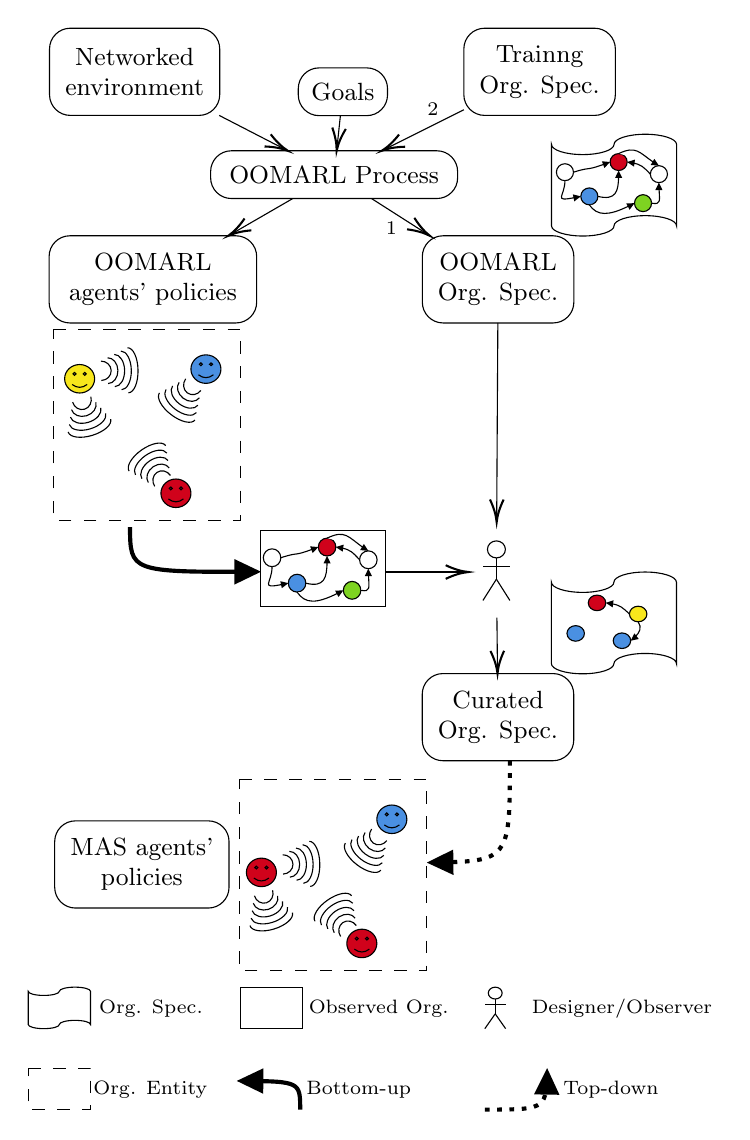
\begin{tikzpicture}[x=0.75pt,y=0.75pt,yscale=-1,xscale=1]
%uncomment if require: \path (0,567); %set diagram left start at 0, and has height of 567

%Flowchart: Punched Tape [id:dp09352793636343182] 
\draw  [fill={rgb, 255:red, 255; green, 255; blue, 255 }  ,fill opacity=1 ] (260,284.9) .. controls (260,287.61) and (266.74,289.81) .. (275.06,289.81) .. controls (283.38,289.81) and (290.12,287.61) .. (290.12,284.9) .. controls (290.12,282.2) and (296.87,280) .. (305.18,280) .. controls (313.5,280) and (320.25,282.2) .. (320.25,284.9) -- (320.25,324.13) .. controls (320.25,321.42) and (313.5,319.23) .. (305.18,319.23) .. controls (296.87,319.23) and (290.12,321.42) .. (290.12,324.13) .. controls (290.12,326.84) and (283.38,329.03) .. (275.06,329.03) .. controls (266.74,329.03) and (260,326.84) .. (260,324.13) -- cycle ;
%Shape: Ellipse [id:dp8537944349912123] 
\draw  [fill={rgb, 255:red, 208; green, 2; blue, 27 }  ,fill opacity=1 ] (277.77,294.86) .. controls (277.77,292.79) and (279.66,291.11) .. (281.98,291.11) .. controls (284.3,291.11) and (286.19,292.79) .. (286.19,294.86) .. controls (286.19,296.94) and (284.3,298.62) .. (281.98,298.62) .. controls (279.66,298.62) and (277.77,296.94) .. (277.77,294.86) -- cycle ;
%Shape: Ellipse [id:dp6897748103188357] 
\draw  [fill={rgb, 255:red, 248; green, 231; blue, 28 }  ,fill opacity=1 ] (297.6,300.23) .. controls (297.6,298.15) and (299.49,296.47) .. (301.81,296.47) .. controls (304.13,296.47) and (306.02,298.15) .. (306.02,300.23) .. controls (306.02,302.3) and (304.13,303.98) .. (301.81,303.98) .. controls (299.49,303.98) and (297.6,302.3) .. (297.6,300.23) -- cycle ;
%Shape: Ellipse [id:dp4802320082509959] 
\draw  [fill={rgb, 255:red, 74; green, 144; blue, 226 }  ,fill opacity=1 ] (289.79,313.09) .. controls (289.79,311.02) and (291.67,309.34) .. (294,309.34) .. controls (296.32,309.34) and (298.2,311.02) .. (298.2,313.09) .. controls (298.2,315.17) and (296.32,316.85) .. (294,316.85) .. controls (291.67,316.85) and (289.79,315.17) .. (289.79,313.09) -- cycle ;
%Curve Lines [id:da7546101861138359] 
\draw [fill={rgb, 255:red, 255; green, 255; blue, 255 }  ,fill opacity=1 ]   (297.6,300.23) .. controls (294.11,296.93) and (293.1,296) .. (289.08,295.29) ;
\draw [shift={(286.19,294.86)}, rotate = 7.39] [fill={rgb, 255:red, 0; green, 0; blue, 0 }  ][line width=0.08]  [draw opacity=0] (3.57,-1.72) -- (0,0) -- (3.57,1.72) -- cycle    ;
%Shape: Ellipse [id:dp693668966316707] 
\draw  [fill={rgb, 255:red, 74; green, 144; blue, 226 }  ,fill opacity=1 ] (267.5,309.58) .. controls (267.5,307.51) and (269.38,305.83) .. (271.71,305.83) .. controls (274.03,305.83) and (275.91,307.51) .. (275.91,309.58) .. controls (275.91,311.65) and (274.03,313.33) .. (271.71,313.33) .. controls (269.38,313.33) and (267.5,311.65) .. (267.5,309.58) -- cycle ;
%Curve Lines [id:da5612242217579502] 
\draw [fill={rgb, 255:red, 255; green, 255; blue, 255 }  ,fill opacity=1 ]   (301.81,303.98) .. controls (303.69,306.69) and (302.57,309.05) .. (300.45,311.16) ;
\draw [shift={(298.2,313.09)}, rotate = 322.38] [fill={rgb, 255:red, 0; green, 0; blue, 0 }  ][line width=0.08]  [draw opacity=0] (3.57,-1.72) -- (0,0) -- (3.57,1.72) -- cycle    ;

%Shape: Rectangle [id:dp7949048767988509] 
\draw  [dash pattern={on 4.5pt off 4.5pt}] (20.05,163.11) -- (110.42,163.11) -- (110.42,255.04) -- (20.05,255.04) -- cycle ;
%Shape: Smiley Face [id:dp8425156316307105] 
\draw  [fill={rgb, 255:red, 248; green, 231; blue, 28 }  ,fill opacity=1 ] (25.48,186.89) .. controls (25.48,183.1) and (28.71,180.03) .. (32.71,180.03) .. controls (36.7,180.03) and (39.94,183.1) .. (39.94,186.89) .. controls (39.94,190.68) and (36.7,193.75) .. (32.71,193.75) .. controls (28.71,193.75) and (25.48,190.68) .. (25.48,186.89) -- cycle ; \draw  [fill={rgb, 255:red, 248; green, 231; blue, 28 }  ,fill opacity=1 ] (29.53,184.56) .. controls (29.53,184.18) and (29.85,183.87) .. (30.25,183.87) .. controls (30.65,183.87) and (30.97,184.18) .. (30.97,184.56) .. controls (30.97,184.94) and (30.65,185.24) .. (30.25,185.24) .. controls (29.85,185.24) and (29.53,184.94) .. (29.53,184.56) -- cycle ; \draw  [fill={rgb, 255:red, 248; green, 231; blue, 28 }  ,fill opacity=1 ] (34.44,184.56) .. controls (34.44,184.18) and (34.77,183.87) .. (35.16,183.87) .. controls (35.56,183.87) and (35.89,184.18) .. (35.89,184.56) .. controls (35.89,184.94) and (35.56,185.24) .. (35.16,185.24) .. controls (34.77,185.24) and (34.44,184.94) .. (34.44,184.56) -- cycle ; \draw   (29.09,189.64) .. controls (31.5,191.47) and (33.91,191.47) .. (36.32,189.64) ;
%Shape: Arc [id:dp7103754459108031] 
\draw  [draw opacity=0] (47.66,206.32) .. controls (47.66,206.32) and (47.66,206.32) .. (47.66,206.32) .. controls (48.43,208.93) and (44.47,212.43) .. (38.81,214.15) .. controls (33.16,215.87) and (27.96,215.15) .. (27.19,212.54) -- (37.43,209.43) -- cycle ; \draw   (47.66,206.32) .. controls (47.66,206.32) and (47.66,206.32) .. (47.66,206.32) .. controls (48.43,208.93) and (44.47,212.43) .. (38.81,214.15) .. controls (33.16,215.87) and (27.96,215.15) .. (27.19,212.54) ;  
%Shape: Arc [id:dp9993647702991559] 
\draw  [draw opacity=0] (45.27,203.61) .. controls (46.04,206.22) and (42.73,209.53) .. (37.89,211) .. controls (33.04,212.48) and (28.49,211.55) .. (27.73,208.94) -- (36.5,206.28) -- cycle ; \draw   (45.27,203.61) .. controls (46.04,206.22) and (42.73,209.53) .. (37.89,211) .. controls (33.04,212.48) and (28.49,211.55) .. (27.73,208.94) ;  
%Shape: Arc [id:dp33021260729129986] 
\draw  [draw opacity=0] (42.88,200.9) .. controls (42.88,200.9) and (42.88,200.9) .. (42.88,200.9) .. controls (43.65,203.51) and (41,206.62) .. (36.96,207.85) .. controls (32.92,209.08) and (29.03,207.96) .. (28.26,205.35) -- (35.57,203.12) -- cycle ; \draw   (42.88,200.9) .. controls (42.88,200.9) and (42.88,200.9) .. (42.88,200.9) .. controls (43.65,203.51) and (41,206.62) .. (36.96,207.85) .. controls (32.92,209.08) and (29.03,207.96) .. (28.26,205.35) ;  
%Shape: Arc [id:dp7515950702187679] 
\draw  [draw opacity=0] (40.5,198.2) .. controls (40.5,198.2) and (40.5,198.2) .. (40.5,198.2) .. controls (40.5,198.2) and (40.5,198.2) .. (40.5,198.2) .. controls (41.26,200.81) and (39.27,203.72) .. (36.04,204.7) .. controls (32.81,205.68) and (29.57,204.36) .. (28.8,201.75) .. controls (28.8,201.75) and (28.8,201.75) .. (28.8,201.75) -- (34.65,199.97) -- cycle ; \draw   (40.5,198.2) .. controls (40.5,198.2) and (40.5,198.2) .. (40.5,198.2) .. controls (40.5,198.2) and (40.5,198.2) .. (40.5,198.2) .. controls (41.26,200.81) and (39.27,203.72) .. (36.04,204.7) .. controls (32.81,205.68) and (29.57,204.36) .. (28.8,201.75) .. controls (28.8,201.75) and (28.8,201.75) .. (28.8,201.75) ;  
%Shape: Arc [id:dp17995425823285305] 
\draw  [draw opacity=0] (38.11,195.49) .. controls (38.11,195.49) and (38.11,195.49) .. (38.11,195.49) .. controls (38.11,195.49) and (38.11,195.49) .. (38.11,195.49) .. controls (38.88,198.1) and (37.53,200.81) .. (35.11,201.55) .. controls (32.69,202.29) and (30.1,200.77) .. (29.34,198.16) -- (33.72,196.82) -- cycle ; \draw   (38.11,195.49) .. controls (38.11,195.49) and (38.11,195.49) .. (38.11,195.49) .. controls (38.11,195.49) and (38.11,195.49) .. (38.11,195.49) .. controls (38.88,198.1) and (37.53,200.81) .. (35.11,201.55) .. controls (32.69,202.29) and (30.1,200.77) .. (29.34,198.16) ;  

%Shape: Arc [id:dp8934563741256025] 
\draw  [draw opacity=0] (55.78,171.93) .. controls (58.46,171.87) and (60.73,176.69) .. (60.84,182.69) .. controls (60.96,188.7) and (58.88,193.6) .. (56.21,193.66) -- (55.99,182.79) -- cycle ; \draw   (55.78,171.93) .. controls (58.46,171.87) and (60.73,176.69) .. (60.84,182.69) .. controls (60.96,188.7) and (58.88,193.6) .. (56.21,193.66) ;  
%Shape: Arc [id:dp5963815446588989] 
\draw  [draw opacity=0] (52.58,173.54) .. controls (55.26,173.49) and (57.51,177.62) .. (57.61,182.76) .. controls (57.71,187.9) and (55.62,192.12) .. (52.94,192.17) -- (52.76,182.86) -- cycle ; \draw   (52.58,173.54) .. controls (55.26,173.49) and (57.51,177.62) .. (57.61,182.76) .. controls (57.71,187.9) and (55.62,192.12) .. (52.94,192.17) ;  
%Shape: Arc [id:dp3378668028957823] 
\draw  [draw opacity=0] (49.38,175.16) .. controls (49.38,175.16) and (49.38,175.16) .. (49.38,175.16) .. controls (49.38,175.16) and (49.38,175.16) .. (49.38,175.16) .. controls (52.06,175.11) and (54.3,178.54) .. (54.38,182.82) .. controls (54.46,187.11) and (52.36,190.63) .. (49.68,190.68) -- (49.53,182.92) -- cycle ; \draw   (49.38,175.16) .. controls (49.38,175.16) and (49.38,175.16) .. (49.38,175.16) .. controls (49.38,175.16) and (49.38,175.16) .. (49.38,175.16) .. controls (52.06,175.11) and (54.3,178.54) .. (54.38,182.82) .. controls (54.46,187.11) and (52.36,190.63) .. (49.68,190.68) ;  
%Shape: Arc [id:dp7870035207223711] 
\draw  [draw opacity=0] (46.18,176.78) .. controls (48.86,176.72) and (51.08,179.46) .. (51.15,182.89) .. controls (51.21,186.32) and (49.1,189.14) .. (46.42,189.2) -- (46.3,182.99) -- cycle ; \draw   (46.18,176.78) .. controls (48.86,176.72) and (51.08,179.46) .. (51.15,182.89) .. controls (51.21,186.32) and (49.1,189.14) .. (46.42,189.2) ;  
%Shape: Arc [id:dp7731275981870975] 
\draw  [draw opacity=0] (42.98,178.39) .. controls (42.98,178.39) and (42.98,178.39) .. (42.98,178.39) .. controls (45.65,178.34) and (47.86,180.38) .. (47.91,182.95) .. controls (47.96,185.53) and (45.83,187.65) .. (43.16,187.71) -- (43.07,183.05) -- cycle ; \draw   (42.98,178.39) .. controls (42.98,178.39) and (42.98,178.39) .. (42.98,178.39) .. controls (45.65,178.34) and (47.86,180.38) .. (47.91,182.95) .. controls (47.96,185.53) and (45.83,187.65) .. (43.16,187.71) ;  

%Shape: Smiley Face [id:dp9460068866596214] 
\draw  [fill={rgb, 255:red, 208; green, 2; blue, 27 }  ,fill opacity=1 ] (71.87,242.05) .. controls (71.87,238.26) and (75.1,235.19) .. (79.1,235.19) .. controls (83.09,235.19) and (86.33,238.26) .. (86.33,242.05) .. controls (86.33,245.84) and (83.09,248.92) .. (79.1,248.92) .. controls (75.1,248.92) and (71.87,245.84) .. (71.87,242.05) -- cycle ; \draw  [fill={rgb, 255:red, 208; green, 2; blue, 27 }  ,fill opacity=1 ] (75.91,239.72) .. controls (75.91,239.34) and (76.24,239.03) .. (76.64,239.03) .. controls (77.04,239.03) and (77.36,239.34) .. (77.36,239.72) .. controls (77.36,240.1) and (77.04,240.4) .. (76.64,240.4) .. controls (76.24,240.4) and (75.91,240.1) .. (75.91,239.72) -- cycle ; \draw  [fill={rgb, 255:red, 208; green, 2; blue, 27 }  ,fill opacity=1 ] (80.83,239.72) .. controls (80.83,239.34) and (81.15,239.03) .. (81.55,239.03) .. controls (81.95,239.03) and (82.28,239.34) .. (82.28,239.72) .. controls (82.28,240.1) and (81.95,240.4) .. (81.55,240.4) .. controls (81.15,240.4) and (80.83,240.1) .. (80.83,239.72) -- cycle ; \draw   (75.48,244.8) .. controls (77.89,246.63) and (80.3,246.63) .. (82.71,244.8) ;
%Shape: Arc [id:dp2662505393390908] 
\draw  [draw opacity=0] (56.53,231.38) .. controls (56.53,231.38) and (56.53,231.38) .. (56.53,231.38) .. controls (56.53,231.38) and (56.53,231.38) .. (56.53,231.38) .. controls (55.02,229.13) and (57.74,224.56) .. (62.6,221.17) .. controls (67.47,217.77) and (72.64,216.84) .. (74.15,219.09) -- (65.34,225.24) -- cycle ; \draw   (56.53,231.38) .. controls (56.53,231.38) and (56.53,231.38) .. (56.53,231.38) .. controls (56.53,231.38) and (56.53,231.38) .. (56.53,231.38) .. controls (55.02,229.13) and (57.74,224.56) .. (62.6,221.17) .. controls (67.47,217.77) and (72.64,216.84) .. (74.15,219.09) ;  
%Shape: Arc [id:dp5533657200850002] 
\draw  [draw opacity=0] (59.62,233.22) .. controls (59.62,233.22) and (59.62,233.22) .. (59.62,233.22) .. controls (58.11,230.97) and (60.26,226.79) .. (64.43,223.88) .. controls (68.6,220.97) and (73.21,220.43) .. (74.72,222.68) -- (67.17,227.95) -- cycle ; \draw   (59.62,233.22) .. controls (59.62,233.22) and (59.62,233.22) .. (59.62,233.22) .. controls (58.11,230.97) and (60.26,226.79) .. (64.43,223.88) .. controls (68.6,220.97) and (73.21,220.43) .. (74.72,222.68) ;  
%Shape: Arc [id:dp130720604660594] 
\draw  [draw opacity=0] (62.71,235.05) .. controls (61.19,232.8) and (62.78,229.02) .. (66.26,226.59) .. controls (69.73,224.17) and (73.78,224.02) .. (75.29,226.27) -- (69,230.66) -- cycle ; \draw   (62.71,235.05) .. controls (61.19,232.8) and (62.78,229.02) .. (66.26,226.59) .. controls (69.73,224.17) and (73.78,224.02) .. (75.29,226.27) ;  
%Shape: Arc [id:dp7777326608896638] 
\draw  [draw opacity=0] (65.79,236.88) .. controls (65.79,236.88) and (65.79,236.88) .. (65.79,236.88) .. controls (64.28,234.64) and (65.31,231.24) .. (68.09,229.3) .. controls (70.87,227.36) and (74.35,227.61) .. (75.86,229.86) -- (70.83,233.37) -- cycle ; \draw   (65.79,236.88) .. controls (65.79,236.88) and (65.79,236.88) .. (65.79,236.88) .. controls (64.28,234.64) and (65.31,231.24) .. (68.09,229.3) .. controls (70.87,227.36) and (74.35,227.61) .. (75.86,229.86) ;  
%Shape: Arc [id:dp4348101062357661] 
\draw  [draw opacity=0] (68.88,238.72) .. controls (67.37,236.47) and (67.83,233.47) .. (69.92,232.02) .. controls (72,230.56) and (74.92,231.2) .. (76.43,233.45) -- (72.66,236.08) -- cycle ; \draw   (68.88,238.72) .. controls (67.37,236.47) and (67.83,233.47) .. (69.92,232.02) .. controls (72,230.56) and (74.92,231.2) .. (76.43,233.45) ;  

%Shape: Smiley Face [id:dp40321958667865143] 
\draw  [fill={rgb, 255:red, 74; green, 144; blue, 226 }  ,fill opacity=1 ] (86.33,182.23) .. controls (86.33,178.44) and (89.56,175.37) .. (93.55,175.37) .. controls (97.55,175.37) and (100.78,178.44) .. (100.78,182.23) .. controls (100.78,186.02) and (97.55,189.1) .. (93.55,189.1) .. controls (89.56,189.1) and (86.33,186.02) .. (86.33,182.23) -- cycle ; \draw  [fill={rgb, 255:red, 74; green, 144; blue, 226 }  ,fill opacity=1 ] (90.37,179.9) .. controls (90.37,179.52) and (90.7,179.21) .. (91.1,179.21) .. controls (91.5,179.21) and (91.82,179.52) .. (91.82,179.9) .. controls (91.82,180.28) and (91.5,180.58) .. (91.1,180.58) .. controls (90.7,180.58) and (90.37,180.28) .. (90.37,179.9) -- cycle ; \draw  [fill={rgb, 255:red, 74; green, 144; blue, 226 }  ,fill opacity=1 ] (95.29,179.9) .. controls (95.29,179.52) and (95.61,179.21) .. (96.01,179.21) .. controls (96.41,179.21) and (96.74,179.52) .. (96.74,179.9) .. controls (96.74,180.28) and (96.41,180.58) .. (96.01,180.58) .. controls (95.61,180.58) and (95.29,180.28) .. (95.29,179.9) -- cycle ; \draw   (89.94,184.98) .. controls (92.35,186.81) and (94.76,186.81) .. (97.17,184.98) ;
%Shape: Arc [id:dp6344973920370733] 
\draw  [draw opacity=0] (88.26,206.75) .. controls (88.26,206.75) and (88.26,206.75) .. (88.26,206.75) .. controls (86.65,208.93) and (81.52,207.78) .. (76.8,204.18) .. controls (72.08,200.58) and (69.55,195.9) .. (71.16,193.72) -- (79.71,200.23) -- cycle ; \draw   (88.26,206.75) .. controls (88.26,206.75) and (88.26,206.75) .. (88.26,206.75) .. controls (86.65,208.93) and (81.52,207.78) .. (76.8,204.18) .. controls (72.08,200.58) and (69.55,195.9) .. (71.16,193.72) ;  
%Shape: Arc [id:dp2502725185770005] 
\draw  [draw opacity=0] (88.97,203.19) .. controls (88.97,203.19) and (88.97,203.19) .. (88.97,203.19) .. controls (88.97,203.19) and (88.97,203.19) .. (88.97,203.19) .. controls (87.37,205.37) and (82.78,204.63) .. (78.74,201.55) .. controls (74.69,198.46) and (72.71,194.2) .. (74.32,192.02) -- (81.65,197.6) -- cycle ; \draw   (88.97,203.19) .. controls (88.97,203.19) and (88.97,203.19) .. (88.97,203.19) .. controls (88.97,203.19) and (88.97,203.19) .. (88.97,203.19) .. controls (87.37,205.37) and (82.78,204.63) .. (78.74,201.55) .. controls (74.69,198.46) and (72.71,194.2) .. (74.32,192.02) ;  
%Shape: Arc [id:dp23421846029392612] 
\draw  [draw opacity=0] (89.69,199.63) .. controls (89.69,199.63) and (89.69,199.63) .. (89.69,199.63) .. controls (89.69,199.63) and (89.69,199.63) .. (89.69,199.63) .. controls (88.08,201.81) and (84.05,201.49) .. (80.68,198.92) .. controls (77.3,196.35) and (75.87,192.5) .. (77.48,190.32) -- (83.58,194.97) -- cycle ; \draw   (89.69,199.63) .. controls (89.69,199.63) and (89.69,199.63) .. (89.69,199.63) .. controls (89.69,199.63) and (89.69,199.63) .. (89.69,199.63) .. controls (88.08,201.81) and (84.05,201.49) .. (80.68,198.92) .. controls (77.3,196.35) and (75.87,192.5) .. (77.48,190.32) ;  
%Shape: Arc [id:dp02946644855410807] 
\draw  [draw opacity=0] (90.41,196.06) .. controls (88.8,198.24) and (85.31,198.34) .. (82.62,196.29) .. controls (79.92,194.23) and (79.03,190.8) .. (80.64,188.62) -- (85.52,192.34) -- cycle ; \draw   (90.41,196.06) .. controls (88.8,198.24) and (85.31,198.34) .. (82.62,196.29) .. controls (79.92,194.23) and (79.03,190.8) .. (80.64,188.62) ;  
%Shape: Arc [id:dp07919277634076938] 
\draw  [draw opacity=0] (91.13,192.5) .. controls (91.13,192.5) and (91.13,192.5) .. (91.13,192.5) .. controls (89.52,194.68) and (86.58,195.2) .. (84.55,193.66) .. controls (82.53,192.11) and (82.19,189.1) .. (83.8,186.92) -- (87.46,189.71) -- cycle ; \draw   (91.13,192.5) .. controls (91.13,192.5) and (91.13,192.5) .. (91.13,192.5) .. controls (89.52,194.68) and (86.58,195.2) .. (84.55,193.66) .. controls (82.53,192.11) and (82.19,189.1) .. (83.8,186.92) ;  

%Shape: Ellipse [id:dp5665300419613197] 
\draw   (229.18,269.1) .. controls (229.18,266.84) and (231.12,265) .. (233.51,265) .. controls (235.9,265) and (237.84,266.84) .. (237.84,269.1) .. controls (237.84,271.36) and (235.9,273.2) .. (233.51,273.2) .. controls (231.12,273.2) and (229.18,271.36) .. (229.18,269.1) -- cycle ;
%Straight Lines [id:da868287133321088] 
\draw    (233.51,273.2) -- (233.51,283.45) ;
%Straight Lines [id:da7338999456859931] 
\draw    (233.51,283.45) -- (227.02,293.7) ;
%Straight Lines [id:da7618645013452761] 
\draw    (233.51,283.45) -- (240,293.7) ;
%Straight Lines [id:da7029210082761028] 
\draw    (240,277.3) -- (227.02,277.3) ;

%Shape: Rectangle [id:dp36259598060414655] 
\draw  [fill={rgb, 255:red, 255; green, 255; blue, 255 }  ,fill opacity=1 ] (120,260) -- (180.25,260) -- (180.25,296.77) -- (120,296.77) -- cycle ;
%Shape: Ellipse [id:dp34598635042601256] 
\draw  [fill={rgb, 255:red, 255; green, 255; blue, 255 }  ,fill opacity=1 ] (121.2,273.12) .. controls (121.2,270.75) and (123.09,268.83) .. (125.42,268.83) .. controls (127.75,268.83) and (129.64,270.75) .. (129.64,273.12) .. controls (129.64,275.49) and (127.75,277.41) .. (125.42,277.41) .. controls (123.09,277.41) and (121.2,275.49) .. (121.2,273.12) -- cycle ;
%Shape: Ellipse [id:dp0011247415244253212] 
\draw  [fill={rgb, 255:red, 74; green, 144; blue, 226 }  ,fill opacity=1 ] (133.25,285.37) .. controls (133.25,283) and (135.14,281.08) .. (137.47,281.08) .. controls (139.8,281.08) and (141.69,283) .. (141.69,285.37) .. controls (141.69,287.74) and (139.8,289.66) .. (137.47,289.66) .. controls (135.14,289.66) and (133.25,287.74) .. (133.25,285.37) -- cycle ;
%Shape: Ellipse [id:dp8822927144483022] 
\draw  [fill={rgb, 255:red, 208; green, 2; blue, 27 }  ,fill opacity=1 ] (147.71,267.97) .. controls (147.71,265.6) and (149.6,263.68) .. (151.93,263.68) .. controls (154.26,263.68) and (156.15,265.6) .. (156.15,267.97) .. controls (156.15,270.34) and (154.26,272.26) .. (151.93,272.26) .. controls (149.6,272.26) and (147.71,270.34) .. (147.71,267.97) -- cycle ;
%Shape: Ellipse [id:dp7611446545020739] 
\draw  [fill={rgb, 255:red, 255; green, 255; blue, 255 }  ,fill opacity=1 ] (167.59,274.1) .. controls (167.59,271.73) and (169.48,269.81) .. (171.81,269.81) .. controls (174.14,269.81) and (176.03,271.73) .. (176.03,274.1) .. controls (176.03,276.47) and (174.14,278.39) .. (171.81,278.39) .. controls (169.48,278.39) and (167.59,276.47) .. (167.59,274.1) -- cycle ;
%Shape: Ellipse [id:dp1592826898001829] 
\draw  [fill={rgb, 255:red, 126; green, 211; blue, 33 }  ,fill opacity=1 ] (159.76,288.81) .. controls (159.76,286.44) and (161.65,284.52) .. (163.98,284.52) .. controls (166.31,284.52) and (168.2,286.44) .. (168.2,288.81) .. controls (168.2,291.18) and (166.31,293.1) .. (163.98,293.1) .. controls (161.65,293.1) and (159.76,291.18) .. (159.76,288.81) -- cycle ;
%Curve Lines [id:da27399536046205264] 
\draw [fill={rgb, 255:red, 255; green, 255; blue, 255 }  ,fill opacity=1 ]   (129.64,273.12) .. controls (139.11,270.05) and (134.67,272.76) .. (144.92,269.01) ;
\draw [shift={(147.71,267.97)}, rotate = 159.17] [fill={rgb, 255:red, 0; green, 0; blue, 0 }  ][line width=0.08]  [draw opacity=0] (3.57,-1.72) -- (0,0) -- (3.57,1.72) -- cycle    ;
%Curve Lines [id:da16623917428090795] 
\draw [fill={rgb, 255:red, 255; green, 255; blue, 255 }  ,fill opacity=1 ]   (141.69,285.37) .. controls (150.75,287.65) and (151.79,282.63) .. (151.91,275.25) ;
\draw [shift={(151.93,272.26)}, rotate = 90] [fill={rgb, 255:red, 0; green, 0; blue, 0 }  ][line width=0.08]  [draw opacity=0] (3.57,-1.72) -- (0,0) -- (3.57,1.72) -- cycle    ;
%Curve Lines [id:da46234775845087284] 
\draw [fill={rgb, 255:red, 255; green, 255; blue, 255 }  ,fill opacity=1 ]   (167.59,274.1) .. controls (164.09,270.33) and (163.08,269.27) .. (159.05,268.46) ;
\draw [shift={(156.15,267.97)}, rotate = 8.42] [fill={rgb, 255:red, 0; green, 0; blue, 0 }  ][line width=0.08]  [draw opacity=0] (3.57,-1.72) -- (0,0) -- (3.57,1.72) -- cycle    ;
%Curve Lines [id:da3119386523209393] 
\draw [fill={rgb, 255:red, 255; green, 255; blue, 255 }  ,fill opacity=1 ]   (168.2,288.81) .. controls (172.97,289.67) and (172.14,287.87) .. (171.87,281.33) ;
\draw [shift={(171.81,278.39)}, rotate = 90] [fill={rgb, 255:red, 0; green, 0; blue, 0 }  ][line width=0.08]  [draw opacity=0] (3.57,-1.72) -- (0,0) -- (3.57,1.72) -- cycle    ;
%Curve Lines [id:da8983756138417751] 
\draw [fill={rgb, 255:red, 255; green, 255; blue, 255 }  ,fill opacity=1 ]   (125.42,277.41) .. controls (125.42,285.5) and (119.17,288.19) .. (130.41,285.96) ;
\draw [shift={(133.25,285.37)}, rotate = 168.05] [fill={rgb, 255:red, 0; green, 0; blue, 0 }  ][line width=0.08]  [draw opacity=0] (3.57,-1.72) -- (0,0) -- (3.57,1.72) -- cycle    ;
%Curve Lines [id:da8579733900345894] 
\draw [fill={rgb, 255:red, 255; green, 255; blue, 255 }  ,fill opacity=1 ]   (137.47,289.66) .. controls (141.37,295.45) and (146.82,295.36) .. (157.15,290.17) ;
\draw [shift={(159.76,288.81)}, rotate = 151.67] [fill={rgb, 255:red, 0; green, 0; blue, 0 }  ][line width=0.08]  [draw opacity=0] (3.57,-1.72) -- (0,0) -- (3.57,1.72) -- cycle    ;
%Curve Lines [id:da598997074659714] 
\draw [fill={rgb, 255:red, 255; green, 255; blue, 255 }  ,fill opacity=1 ]   (151.93,263.68) .. controls (160.7,259.44) and (161.99,263.12) .. (169.42,268.25) ;
\draw [shift={(171.81,269.81)}, rotate = 211.4] [fill={rgb, 255:red, 0; green, 0; blue, 0 }  ][line width=0.08]  [draw opacity=0] (3.57,-1.72) -- (0,0) -- (3.57,1.72) -- cycle    ;

%Shape: Boxed Bezier Curve [id:dp04329100663395624] 
\draw [line width=1.5]    (56.97,258.4) .. controls (57.12,279.64) and (57.12,280.06) .. (116.36,279.88) ;
\draw [shift={(120.07,279.86)}, rotate = 179.81] [fill={rgb, 255:red, 0; green, 0; blue, 0 }  ][line width=0.08]  [draw opacity=0] (12.77,-6.13) -- (0,0) -- (12.77,6.13) -- cycle    ;
%Shape: Boxed Bezier Curve [id:dp3249540323733473] 
\draw [line width=1.5]  [dash pattern={on 1.69pt off 2.76pt}]  (240,371) .. controls (240,377.31) and (240,382.8) .. (239.91,387.58) .. controls (239.34,418.4) and (235.11,419.53) .. (203.54,419.96) ;
\draw [shift={(200,420)}, rotate = 359.3] [fill={rgb, 255:red, 0; green, 0; blue, 0 }  ][line width=0.08]  [draw opacity=0] (12.77,-6.13) -- (0,0) -- (12.77,6.13) -- cycle    ;
%Shape: Rectangle [id:dp3591393250200341] 
\draw  [dash pattern={on 4.5pt off 4.5pt}] (109.63,380) -- (200,380) -- (200,471.94) -- (109.63,471.94) -- cycle ;
%Shape: Smiley Face [id:dp3801591887945033] 
\draw  [fill={rgb, 255:red, 208; green, 2; blue, 27 }  ,fill opacity=1 ] (113.05,424.72) .. controls (113.05,420.92) and (116.29,417.85) .. (120.28,417.85) .. controls (124.28,417.85) and (127.51,420.92) .. (127.51,424.72) .. controls (127.51,428.51) and (124.28,431.58) .. (120.28,431.58) .. controls (116.29,431.58) and (113.05,428.51) .. (113.05,424.72) -- cycle ; \draw  [fill={rgb, 255:red, 208; green, 2; blue, 27 }  ,fill opacity=1 ] (117.1,422.38) .. controls (117.1,422) and (117.43,421.7) .. (117.82,421.7) .. controls (118.22,421.7) and (118.55,422) .. (118.55,422.38) .. controls (118.55,422.76) and (118.22,423.07) .. (117.82,423.07) .. controls (117.43,423.07) and (117.1,422.76) .. (117.1,422.38) -- cycle ; \draw  [fill={rgb, 255:red, 208; green, 2; blue, 27 }  ,fill opacity=1 ] (122.02,422.38) .. controls (122.02,422) and (122.34,421.7) .. (122.74,421.7) .. controls (123.14,421.7) and (123.46,422) .. (123.46,422.38) .. controls (123.46,422.76) and (123.14,423.07) .. (122.74,423.07) .. controls (122.34,423.07) and (122.02,422.76) .. (122.02,422.38) -- cycle ; \draw   (116.67,427.46) .. controls (119.08,429.29) and (121.49,429.29) .. (123.9,427.46) ;
%Shape: Arc [id:dp40222913228483237] 
\draw  [draw opacity=0] (135.24,444.14) .. controls (135.24,444.14) and (135.24,444.14) .. (135.24,444.14) .. controls (136,446.75) and (132.04,450.26) .. (126.39,451.98) .. controls (120.74,453.7) and (115.53,452.97) .. (114.77,450.36) -- (125,447.25) -- cycle ; \draw   (135.24,444.14) .. controls (135.24,444.14) and (135.24,444.14) .. (135.24,444.14) .. controls (136,446.75) and (132.04,450.26) .. (126.39,451.98) .. controls (120.74,453.7) and (115.53,452.97) .. (114.77,450.36) ;  
%Shape: Arc [id:dp6185790641450695] 
\draw  [draw opacity=0] (132.85,441.43) .. controls (133.62,444.05) and (130.31,447.36) .. (125.46,448.83) .. controls (120.62,450.3) and (116.07,449.38) .. (115.3,446.77) -- (124.08,444.1) -- cycle ; \draw   (132.85,441.43) .. controls (133.62,444.05) and (130.31,447.36) .. (125.46,448.83) .. controls (120.62,450.3) and (116.07,449.38) .. (115.3,446.77) ;  
%Shape: Arc [id:dp6749114191148724] 
\draw  [draw opacity=0] (130.46,438.73) .. controls (130.46,438.73) and (130.46,438.73) .. (130.46,438.73) .. controls (131.23,441.34) and (128.58,444.45) .. (124.54,445.68) .. controls (120.5,446.9) and (116.61,445.78) .. (115.84,443.17) -- (123.15,440.95) -- cycle ; \draw   (130.46,438.73) .. controls (130.46,438.73) and (130.46,438.73) .. (130.46,438.73) .. controls (131.23,441.34) and (128.58,444.45) .. (124.54,445.68) .. controls (120.5,446.9) and (116.61,445.78) .. (115.84,443.17) ;  
%Shape: Arc [id:dp056403546095020296] 
\draw  [draw opacity=0] (128.07,436.02) .. controls (128.07,436.02) and (128.07,436.02) .. (128.07,436.02) .. controls (128.07,436.02) and (128.07,436.02) .. (128.07,436.02) .. controls (128.84,438.63) and (126.84,441.54) .. (123.61,442.53) .. controls (120.38,443.51) and (117.14,442.19) .. (116.38,439.58) -- (122.22,437.8) -- cycle ; \draw   (128.07,436.02) .. controls (128.07,436.02) and (128.07,436.02) .. (128.07,436.02) .. controls (128.07,436.02) and (128.07,436.02) .. (128.07,436.02) .. controls (128.84,438.63) and (126.84,441.54) .. (123.61,442.53) .. controls (120.38,443.51) and (117.14,442.19) .. (116.38,439.58) ;  
%Shape: Arc [id:dp048963270262922354] 
\draw  [draw opacity=0] (125.69,433.32) .. controls (125.69,433.32) and (125.69,433.32) .. (125.69,433.32) .. controls (126.45,435.93) and (125.11,438.64) .. (122.69,439.38) .. controls (120.27,440.11) and (117.68,438.59) .. (116.91,435.98) -- (121.3,434.65) -- cycle ; \draw   (125.69,433.32) .. controls (125.69,433.32) and (125.69,433.32) .. (125.69,433.32) .. controls (126.45,435.93) and (125.11,438.64) .. (122.69,439.38) .. controls (120.27,440.11) and (117.68,438.59) .. (116.91,435.98) ;  

%Shape: Arc [id:dp11791815378481285] 
\draw  [draw opacity=0] (143.36,409.75) .. controls (143.36,409.75) and (143.36,409.75) .. (143.36,409.75) .. controls (146.04,409.7) and (148.3,414.52) .. (148.42,420.52) .. controls (148.54,426.52) and (146.46,431.43) .. (143.78,431.48) -- (143.57,420.62) -- cycle ; \draw   (143.36,409.75) .. controls (143.36,409.75) and (143.36,409.75) .. (143.36,409.75) .. controls (146.04,409.7) and (148.3,414.52) .. (148.42,420.52) .. controls (148.54,426.52) and (146.46,431.43) .. (143.78,431.48) ;  
%Shape: Arc [id:dp6186444432706435] 
\draw  [draw opacity=0] (140.16,411.37) .. controls (142.84,411.32) and (145.09,415.44) .. (145.19,420.59) .. controls (145.29,425.73) and (143.2,429.94) .. (140.52,430) -- (140.34,420.68) -- cycle ; \draw   (140.16,411.37) .. controls (142.84,411.32) and (145.09,415.44) .. (145.19,420.59) .. controls (145.29,425.73) and (143.2,429.94) .. (140.52,430) ;  
%Shape: Arc [id:dp3524256769019909] 
\draw  [draw opacity=0] (136.96,412.99) .. controls (136.96,412.99) and (136.96,412.99) .. (136.96,412.99) .. controls (139.63,412.93) and (141.87,416.36) .. (141.96,420.65) .. controls (142.04,424.94) and (139.94,428.45) .. (137.26,428.51) .. controls (137.26,428.51) and (137.26,428.51) .. (137.26,428.51) -- (137.11,420.75) -- cycle ; \draw   (136.96,412.99) .. controls (136.96,412.99) and (136.96,412.99) .. (136.96,412.99) .. controls (139.63,412.93) and (141.87,416.36) .. (141.96,420.65) .. controls (142.04,424.94) and (139.94,428.45) .. (137.26,428.51) .. controls (137.26,428.51) and (137.26,428.51) .. (137.26,428.51) ;  
%Shape: Arc [id:dp9364872182962407] 
\draw  [draw opacity=0] (133.76,414.6) .. controls (136.43,414.55) and (138.66,417.29) .. (138.72,420.72) .. controls (138.79,424.14) and (136.67,426.97) .. (134,427.02) -- (133.88,420.81) -- cycle ; \draw   (133.76,414.6) .. controls (136.43,414.55) and (138.66,417.29) .. (138.72,420.72) .. controls (138.79,424.14) and (136.67,426.97) .. (134,427.02) ;  
%Shape: Arc [id:dp43568764349824574] 
\draw  [draw opacity=0] (130.55,416.22) .. controls (130.55,416.22) and (130.55,416.22) .. (130.55,416.22) .. controls (133.23,416.17) and (135.44,418.21) .. (135.49,420.78) .. controls (135.54,423.35) and (133.41,425.48) .. (130.73,425.53) .. controls (130.73,425.53) and (130.73,425.53) .. (130.73,425.53) -- (130.64,420.88) -- cycle ; \draw   (130.55,416.22) .. controls (130.55,416.22) and (130.55,416.22) .. (130.55,416.22) .. controls (133.23,416.17) and (135.44,418.21) .. (135.49,420.78) .. controls (135.54,423.35) and (133.41,425.48) .. (130.73,425.53) .. controls (130.73,425.53) and (130.73,425.53) .. (130.73,425.53) ;  

%Shape: Smiley Face [id:dp7641236455099758] 
\draw  [fill={rgb, 255:red, 208; green, 2; blue, 27 }  ,fill opacity=1 ] (161.44,458.94) .. controls (161.44,455.15) and (164.68,452.08) .. (168.67,452.08) .. controls (172.66,452.08) and (175.9,455.15) .. (175.9,458.94) .. controls (175.9,462.73) and (172.66,465.81) .. (168.67,465.81) .. controls (164.68,465.81) and (161.44,462.73) .. (161.44,458.94) -- cycle ; \draw  [fill={rgb, 255:red, 208; green, 2; blue, 27 }  ,fill opacity=1 ] (165.49,456.61) .. controls (165.49,456.23) and (165.81,455.92) .. (166.21,455.92) .. controls (166.61,455.92) and (166.94,456.23) .. (166.94,456.61) .. controls (166.94,456.99) and (166.61,457.29) .. (166.21,457.29) .. controls (165.81,457.29) and (165.49,456.99) .. (165.49,456.61) -- cycle ; \draw  [fill={rgb, 255:red, 208; green, 2; blue, 27 }  ,fill opacity=1 ] (170.41,456.61) .. controls (170.41,456.23) and (170.73,455.92) .. (171.13,455.92) .. controls (171.53,455.92) and (171.85,456.23) .. (171.85,456.61) .. controls (171.85,456.99) and (171.53,457.29) .. (171.13,457.29) .. controls (170.73,457.29) and (170.41,456.99) .. (170.41,456.61) -- cycle ; \draw   (165.06,461.69) .. controls (167.47,463.52) and (169.88,463.52) .. (172.29,461.69) ;
%Shape: Arc [id:dp12338485660705834] 
\draw  [draw opacity=0] (146.11,448.27) .. controls (146.11,448.27) and (146.11,448.27) .. (146.11,448.27) .. controls (144.6,446.02) and (147.31,441.45) .. (152.18,438.06) .. controls (157.04,434.66) and (162.22,433.73) .. (163.73,435.98) -- (154.92,442.13) -- cycle ; \draw   (146.11,448.27) .. controls (146.11,448.27) and (146.11,448.27) .. (146.11,448.27) .. controls (144.6,446.02) and (147.31,441.45) .. (152.18,438.06) .. controls (157.04,434.66) and (162.22,433.73) .. (163.73,435.98) ;  
%Shape: Arc [id:dp047340824310728946] 
\draw  [draw opacity=0] (149.2,450.11) .. controls (149.2,450.11) and (149.2,450.11) .. (149.2,450.11) .. controls (147.68,447.86) and (149.84,443.68) .. (154.01,440.77) .. controls (158.18,437.86) and (162.79,437.32) .. (164.3,439.57) -- (156.75,444.84) -- cycle ; \draw   (149.2,450.11) .. controls (149.2,450.11) and (149.2,450.11) .. (149.2,450.11) .. controls (147.68,447.86) and (149.84,443.68) .. (154.01,440.77) .. controls (158.18,437.86) and (162.79,437.32) .. (164.3,439.57) ;  
%Shape: Arc [id:dp5460583680593605] 
\draw  [draw opacity=0] (152.28,451.94) .. controls (150.77,449.69) and (152.36,445.91) .. (155.84,443.48) .. controls (159.31,441.06) and (163.36,440.91) .. (164.87,443.16) -- (158.58,447.55) -- cycle ; \draw   (152.28,451.94) .. controls (150.77,449.69) and (152.36,445.91) .. (155.84,443.48) .. controls (159.31,441.06) and (163.36,440.91) .. (164.87,443.16) ;  
%Shape: Arc [id:dp9281425971103023] 
\draw  [draw opacity=0] (155.37,453.77) .. controls (155.37,453.77) and (155.37,453.77) .. (155.37,453.77) .. controls (153.86,451.53) and (154.88,448.13) .. (157.66,446.19) .. controls (160.44,444.25) and (163.93,444.5) .. (165.44,446.75) -- (160.41,450.26) -- cycle ; \draw   (155.37,453.77) .. controls (155.37,453.77) and (155.37,453.77) .. (155.37,453.77) .. controls (153.86,451.53) and (154.88,448.13) .. (157.66,446.19) .. controls (160.44,444.25) and (163.93,444.5) .. (165.44,446.75) ;  
%Shape: Arc [id:dp6708756452099565] 
\draw  [draw opacity=0] (158.46,455.61) .. controls (158.46,455.61) and (158.46,455.61) .. (158.46,455.61) .. controls (156.94,453.36) and (157.41,450.36) .. (159.49,448.91) .. controls (161.58,447.45) and (164.49,448.09) .. (166.01,450.34) -- (162.23,452.98) -- cycle ; \draw   (158.46,455.61) .. controls (158.46,455.61) and (158.46,455.61) .. (158.46,455.61) .. controls (156.94,453.36) and (157.41,450.36) .. (159.49,448.91) .. controls (161.58,447.45) and (164.49,448.09) .. (166.01,450.34) ;  

%Shape: Smiley Face [id:dp8284136369467816] 
\draw  [fill={rgb, 255:red, 74; green, 144; blue, 226 }  ,fill opacity=1 ] (175.9,399.12) .. controls (175.9,395.33) and (179.14,392.26) .. (183.13,392.26) .. controls (187.12,392.26) and (190.36,395.33) .. (190.36,399.12) .. controls (190.36,402.91) and (187.12,405.99) .. (183.13,405.99) .. controls (179.14,405.99) and (175.9,402.91) .. (175.9,399.12) -- cycle ; \draw  [fill={rgb, 255:red, 74; green, 144; blue, 226 }  ,fill opacity=1 ] (179.95,396.79) .. controls (179.95,396.41) and (180.27,396.1) .. (180.67,396.1) .. controls (181.07,396.1) and (181.4,396.41) .. (181.4,396.79) .. controls (181.4,397.17) and (181.07,397.48) .. (180.67,397.48) .. controls (180.27,397.48) and (179.95,397.17) .. (179.95,396.79) -- cycle ; \draw  [fill={rgb, 255:red, 74; green, 144; blue, 226 }  ,fill opacity=1 ] (184.87,396.79) .. controls (184.87,396.41) and (185.19,396.1) .. (185.59,396.1) .. controls (185.99,396.1) and (186.31,396.41) .. (186.31,396.79) .. controls (186.31,397.17) and (185.99,397.48) .. (185.59,397.48) .. controls (185.19,397.48) and (184.87,397.17) .. (184.87,396.79) -- cycle ; \draw   (179.52,401.87) .. controls (181.93,403.7) and (184.34,403.7) .. (186.75,401.87) ;
%Shape: Arc [id:dp8977395703020796] 
\draw  [draw opacity=0] (177.83,423.64) .. controls (177.83,423.64) and (177.83,423.64) .. (177.83,423.64) .. controls (176.23,425.82) and (171.1,424.67) .. (166.38,421.07) .. controls (161.66,417.47) and (159.13,412.79) .. (160.74,410.61) -- (169.28,417.13) -- cycle ; \draw   (177.83,423.64) .. controls (177.83,423.64) and (177.83,423.64) .. (177.83,423.64) .. controls (176.23,425.82) and (171.1,424.67) .. (166.38,421.07) .. controls (161.66,417.47) and (159.13,412.79) .. (160.74,410.61) ;  
%Shape: Arc [id:dp38070292756653834] 
\draw  [draw opacity=0] (178.55,420.08) .. controls (178.55,420.08) and (178.55,420.08) .. (178.55,420.08) .. controls (178.55,420.08) and (178.55,420.08) .. (178.55,420.08) .. controls (176.94,422.26) and (172.36,421.53) .. (168.31,418.44) .. controls (164.27,415.36) and (162.29,411.09) .. (163.9,408.91) -- (171.22,414.49) -- cycle ; \draw   (178.55,420.08) .. controls (178.55,420.08) and (178.55,420.08) .. (178.55,420.08) .. controls (178.55,420.08) and (178.55,420.08) .. (178.55,420.08) .. controls (176.94,422.26) and (172.36,421.53) .. (168.31,418.44) .. controls (164.27,415.36) and (162.29,411.09) .. (163.9,408.91) ;  
%Shape: Arc [id:dp6719893406275441] 
\draw  [draw opacity=0] (179.27,416.52) .. controls (177.66,418.7) and (173.63,418.38) .. (170.25,415.81) .. controls (166.88,413.24) and (165.45,409.39) .. (167.06,407.21) -- (173.16,411.86) -- cycle ; \draw   (179.27,416.52) .. controls (177.66,418.7) and (173.63,418.38) .. (170.25,415.81) .. controls (166.88,413.24) and (165.45,409.39) .. (167.06,407.21) ;  
%Shape: Arc [id:dp8811123580129818] 
\draw  [draw opacity=0] (179.98,412.95) .. controls (178.38,415.13) and (174.89,415.23) .. (172.19,413.18) .. controls (169.49,411.12) and (168.61,407.69) .. (170.22,405.51) -- (175.1,409.23) -- cycle ; \draw   (179.98,412.95) .. controls (178.38,415.13) and (174.89,415.23) .. (172.19,413.18) .. controls (169.49,411.12) and (168.61,407.69) .. (170.22,405.51) ;  
%Shape: Arc [id:dp008168376750506745] 
\draw  [draw opacity=0] (180.7,409.39) .. controls (179.1,411.57) and (176.15,412.09) .. (174.13,410.55) .. controls (172.11,409) and (171.77,405.99) .. (173.38,403.81) -- (177.04,406.6) -- cycle ; \draw   (180.7,409.39) .. controls (179.1,411.57) and (176.15,412.09) .. (174.13,410.55) .. controls (172.11,409) and (171.77,405.99) .. (173.38,403.81) ;  

%Flowchart: Punched Tape [id:dp3402123777548822] 
\draw  [fill={rgb, 255:red, 255; green, 255; blue, 255 }  ,fill opacity=1 ] (7.94,482) .. controls (7.94,483.1) and (11.3,484) .. (15.44,484) .. controls (19.58,484) and (22.94,483.1) .. (22.94,482) .. controls (22.94,480.9) and (26.3,480) .. (30.44,480) .. controls (34.58,480) and (37.94,480.9) .. (37.94,482) -- (37.94,498) .. controls (37.94,496.9) and (34.58,496) .. (30.44,496) .. controls (26.3,496) and (22.94,496.9) .. (22.94,498) .. controls (22.94,499.1) and (19.58,500) .. (15.44,500) .. controls (11.3,500) and (7.94,499.1) .. (7.94,498) -- cycle ;
%Shape: Rectangle [id:dp5542564540555983] 
\draw  [dash pattern={on 4.5pt off 4.5pt}] (7.94,519) -- (37.94,519) -- (37.94,539) -- (7.94,539) -- cycle ;
%Shape: Ellipse [id:dp5593235195310067] 
\draw   (229.6,482.86) .. controls (229.6,481.28) and (231.1,480) .. (232.94,480) .. controls (234.78,480) and (236.27,481.28) .. (236.27,482.86) .. controls (236.27,484.44) and (234.78,485.71) .. (232.94,485.71) .. controls (231.1,485.71) and (229.6,484.44) .. (229.6,482.86) -- cycle ;
%Straight Lines [id:da12195011989321491] 
\draw    (232.94,485.71) -- (232.94,492.86) ;
%Straight Lines [id:da9713687192344966] 
\draw    (232.94,492.86) -- (227.94,500) ;
%Straight Lines [id:da9227495247808029] 
\draw    (232.94,492.86) -- (237.94,500) ;
%Straight Lines [id:da9436032646867678] 
\draw    (237.94,488.57) -- (227.94,488.57) ;

%Shape: Boxed Bezier Curve [id:dp6746038394007414] 
\draw [line width=1.5]  [dash pattern={on 1.69pt off 2.76pt}]  (227.94,539) .. controls (255.56,539) and (257.49,539) .. (257.87,522.91) ;
\draw [shift={(257.94,519)}, rotate = 90.86] [fill={rgb, 255:red, 0; green, 0; blue, 0 }  ][line width=0.08]  [draw opacity=0] (12.77,-6.13) -- (0,0) -- (12.77,6.13) -- cycle    ;
%Shape: Boxed Bezier Curve [id:dp8252767880244336] 
\draw [line width=1.5]    (138.97,539) .. controls (138.97,525.94) and (138.97,525.35) .. (112.36,525.2) ;
\draw [shift={(108.42,525.18)}, rotate = 0.26] [fill={rgb, 255:red, 0; green, 0; blue, 0 }  ][line width=0.08]  [draw opacity=0] (12.77,-6.13) -- (0,0) -- (12.77,6.13) -- cycle    ;
%Flowchart: Punched Tape [id:dp1596519476860545] 
\draw  [fill={rgb, 255:red, 255; green, 255; blue, 255 }  ,fill opacity=1 ] (260.05,73.98) .. controls (260.05,76.69) and (266.8,78.88) .. (275.12,78.88) .. controls (283.43,78.88) and (290.18,76.69) .. (290.18,73.98) .. controls (290.18,71.27) and (296.92,69.08) .. (305.24,69.08) .. controls (313.56,69.08) and (320.3,71.27) .. (320.3,73.98) -- (320.3,113.21) .. controls (320.3,110.5) and (313.56,108.3) .. (305.24,108.3) .. controls (296.92,108.3) and (290.18,110.5) .. (290.18,113.21) .. controls (290.18,115.91) and (283.43,118.11) .. (275.12,118.11) .. controls (266.8,118.11) and (260.05,115.91) .. (260.05,113.21) -- cycle ;
%Shape: Ellipse [id:dp002685494295735058] 
\draw  [fill={rgb, 255:red, 255; green, 255; blue, 255 }  ,fill opacity=1 ] (262.41,87.37) .. controls (262.41,85.11) and (264.25,83.29) .. (266.52,83.29) .. controls (268.8,83.29) and (270.64,85.11) .. (270.64,87.37) .. controls (270.64,89.62) and (268.8,91.44) .. (266.52,91.44) .. controls (264.25,91.44) and (262.41,89.62) .. (262.41,87.37) -- cycle ;
%Shape: Ellipse [id:dp18321883985201803] 
\draw  [fill={rgb, 255:red, 74; green, 144; blue, 226 }  ,fill opacity=1 ] (274.17,99.02) .. controls (274.17,96.76) and (276.01,94.94) .. (278.28,94.94) .. controls (280.56,94.94) and (282.4,96.76) .. (282.4,99.02) .. controls (282.4,101.27) and (280.56,103.09) .. (278.28,103.09) .. controls (276.01,103.09) and (274.17,101.27) .. (274.17,99.02) -- cycle ;
%Shape: Ellipse [id:dp4076602785297232] 
\draw  [fill={rgb, 255:red, 208; green, 2; blue, 27 }  ,fill opacity=1 ] (288.28,82.47) .. controls (288.28,80.22) and (290.12,78.4) .. (292.4,78.4) .. controls (294.67,78.4) and (296.51,80.22) .. (296.51,82.47) .. controls (296.51,84.73) and (294.67,86.55) .. (292.4,86.55) .. controls (290.12,86.55) and (288.28,84.73) .. (288.28,82.47) -- cycle ;
%Shape: Ellipse [id:dp9213295790384606] 
\draw  [fill={rgb, 255:red, 255; green, 255; blue, 255 }  ,fill opacity=1 ] (307.68,88.3) .. controls (307.68,86.05) and (309.53,84.22) .. (311.8,84.22) .. controls (314.07,84.22) and (315.92,86.05) .. (315.92,88.3) .. controls (315.92,90.55) and (314.07,92.38) .. (311.8,92.38) .. controls (309.53,92.38) and (307.68,90.55) .. (307.68,88.3) -- cycle ;
%Shape: Ellipse [id:dp07303077783269196] 
\draw  [fill={rgb, 255:red, 126; green, 211; blue, 33 }  ,fill opacity=1 ] (300.04,102.28) .. controls (300.04,100.03) and (301.88,98.2) .. (304.16,98.2) .. controls (306.43,98.2) and (308.27,100.03) .. (308.27,102.28) .. controls (308.27,104.53) and (306.43,106.35) .. (304.16,106.35) .. controls (301.88,106.35) and (300.04,104.53) .. (300.04,102.28) -- cycle ;
%Curve Lines [id:da40084119138850793] 
\draw [fill={rgb, 255:red, 255; green, 255; blue, 255 }  ,fill opacity=1 ]   (270.64,87.37) .. controls (279.89,84.46) and (275.55,87.03) .. (285.55,83.47) ;
\draw [shift={(288.28,82.47)}, rotate = 159.68] [fill={rgb, 255:red, 0; green, 0; blue, 0 }  ][line width=0.08]  [draw opacity=0] (3.57,-1.72) -- (0,0) -- (3.57,1.72) -- cycle    ;
%Curve Lines [id:da056316075040988345] 
\draw [fill={rgb, 255:red, 255; green, 255; blue, 255 }  ,fill opacity=1 ]   (282.4,99.02) .. controls (291.2,101.17) and (292.25,96.46) .. (292.38,89.51) ;
\draw [shift={(292.4,86.55)}, rotate = 90] [fill={rgb, 255:red, 0; green, 0; blue, 0 }  ][line width=0.08]  [draw opacity=0] (3.57,-1.72) -- (0,0) -- (3.57,1.72) -- cycle    ;
%Curve Lines [id:da9750985583942122] 
\draw [fill={rgb, 255:red, 255; green, 255; blue, 255 }  ,fill opacity=1 ]   (307.68,88.3) .. controls (304.29,84.74) and (303.29,83.72) .. (299.42,82.95) ;
\draw [shift={(296.51,82.47)}, rotate = 8.2] [fill={rgb, 255:red, 0; green, 0; blue, 0 }  ][line width=0.08]  [draw opacity=0] (3.57,-1.72) -- (0,0) -- (3.57,1.72) -- cycle    ;
%Curve Lines [id:da6143174667543494] 
\draw [fill={rgb, 255:red, 255; green, 255; blue, 255 }  ,fill opacity=1 ]   (308.27,102.28) .. controls (312.9,103.09) and (312.13,101.41) .. (311.87,95.28) ;
\draw [shift={(311.8,92.38)}, rotate = 90] [fill={rgb, 255:red, 0; green, 0; blue, 0 }  ][line width=0.08]  [draw opacity=0] (3.57,-1.72) -- (0,0) -- (3.57,1.72) -- cycle    ;
%Curve Lines [id:da2385044516658259] 
\draw [fill={rgb, 255:red, 255; green, 255; blue, 255 }  ,fill opacity=1 ]   (266.52,91.44) .. controls (266.52,99.14) and (260.42,101.69) .. (271.39,99.57) ;
\draw [shift={(274.17,99.02)}, rotate = 168.36] [fill={rgb, 255:red, 0; green, 0; blue, 0 }  ][line width=0.08]  [draw opacity=0] (3.57,-1.72) -- (0,0) -- (3.57,1.72) -- cycle    ;
%Curve Lines [id:da43759757255400467] 
\draw [fill={rgb, 255:red, 255; green, 255; blue, 255 }  ,fill opacity=1 ]   (278.28,103.09) .. controls (282.09,108.59) and (287.41,108.5) .. (297.49,103.57) ;
\draw [shift={(300.04,102.28)}, rotate = 152.3] [fill={rgb, 255:red, 0; green, 0; blue, 0 }  ][line width=0.08]  [draw opacity=0] (3.57,-1.72) -- (0,0) -- (3.57,1.72) -- cycle    ;
%Curve Lines [id:da6953413668483659] 
\draw [fill={rgb, 255:red, 255; green, 255; blue, 255 }  ,fill opacity=1 ]   (292.4,78.4) .. controls (300.91,74.39) and (302.2,77.83) .. (309.34,82.66) ;
\draw [shift={(311.8,84.22)}, rotate = 210.72] [fill={rgb, 255:red, 0; green, 0; blue, 0 }  ][line width=0.08]  [draw opacity=0] (3.57,-1.72) -- (0,0) -- (3.57,1.72) -- cycle    ;

%Shape: Rectangle [id:dp9331446837705206] 
\draw   (110.07,480) -- (140.07,480) -- (140.07,500) -- (110.07,500) -- cycle ;
%Straight Lines [id:da26229660491858264] 
\draw    (180,280) -- (218,280) ;
\draw [shift={(220,280)}, rotate = 180] [color={rgb, 255:red, 0; green, 0; blue, 0 }  ][line width=0.75]    (10.93,-3.29) .. controls (6.95,-1.4) and (3.31,-0.3) .. (0,0) .. controls (3.31,0.3) and (6.95,1.4) .. (10.93,3.29)   ;


% Text Node
\draw (176.81,490.5) node   [align=left] {{\scriptsize Observed Org.}};
% Text Node
\draw    (197.77,338.92) .. controls (197.77,333.4) and (202.24,328.92) .. (207.77,328.92) -- (260.77,328.92) .. controls (266.29,328.92) and (270.77,333.4) .. (270.77,338.92) -- (270.77,360.92) .. controls (270.77,366.45) and (266.29,370.92) .. (260.77,370.92) -- (207.77,370.92) .. controls (202.24,370.92) and (197.77,366.45) .. (197.77,360.92) -- cycle  ;
\draw (234.27,349.92) node  [font=\small] [align=left] {\begin{minipage}[lt]{46.6pt}\setlength\topsep{0pt}
\begin{center}
Curated\\Org. Spec.
\end{center}

\end{minipage}};
% Text Node
\draw (288.7,529.5) node   [align=left] {{\scriptsize Top-down}};
% Text Node
\draw (167.19,529.5) node   [align=left] {{\scriptsize Bottom-up}};
% Text Node
\draw (294,490.5) node   [align=left] {{\scriptsize Designer/Observer}};
% Text Node
\draw (66.74,529.5) node   [align=left] {{\scriptsize Org. Entity}};
% Text Node
\draw (67.04,490.5) node   [align=left] {{\scriptsize Org. Spec.}};
% Text Node
\draw (199,53) node [anchor=north west][inner sep=0.75pt]   [align=left] {$\displaystyle ^{2}$};
% Text Node
% \draw (179,97) node [anchor=north west][inner sep=0.75pt]   [align=left] {$\displaystyle ^{1}$};
\draw (179,110) node [anchor=north west][inner sep=0.75pt]   [align=left] {$\displaystyle ^{1}$};
% Text Node
\draw    (20.69,409.89) .. controls (20.69,404.37) and (25.17,399.89) .. (30.69,399.89) -- (94.69,399.89) .. controls (100.22,399.89) and (104.69,404.37) .. (104.69,409.89) -- (104.69,431.89) .. controls (104.69,437.41) and (100.22,441.89) .. (94.69,441.89) -- (30.69,441.89) .. controls (25.17,441.89) and (20.69,437.41) .. (20.69,431.89) -- cycle  ;
\draw (62.69,420.89) node  [font=\small] [align=left] {\begin{minipage}[lt]{54.49pt}\setlength\topsep{0pt}
\begin{center}
MAS agents'\\policies
\end{center}

\end{minipage}};
% Text Node
\draw (226,257) node [anchor=north west][inner sep=0.75pt]   [align=left] {\begin{minipage}[lt]{8.67pt}\setlength\topsep{0pt}
\begin{center}
\
\end{center}

\end{minipage}};
% Text Node
\draw    (197.82,128) .. controls (197.82,122.48) and (202.3,118) .. (207.82,118) -- (260.82,118) .. controls (266.34,118) and (270.82,122.48) .. (270.82,128) -- (270.82,150) .. controls (270.82,155.52) and (266.34,160) .. (260.82,160) -- (207.82,160) .. controls (202.3,160) and (197.82,155.52) .. (197.82,150) -- cycle  ;
\draw (234.32,139) node  [font=\small] [align=left] {\begin{minipage}[lt]{46.6pt}\setlength\topsep{0pt}
\begin{center}
OOMARL\\Org. Spec.
\end{center}

\end{minipage}};
% Text Node
\draw    (18,128) .. controls (18,122.48) and (22.48,118) .. (28,118) -- (108,118) .. controls (113.52,118) and (118,122.48) .. (118,128) -- (118,150) .. controls (118,155.52) and (113.52,160) .. (108,160) -- (28,160) .. controls (22.48,160) and (18,155.52) .. (18,150) -- cycle  ;
\draw (68,139) node  [font=\small] [align=left] {\begin{minipage}[lt]{65.21pt}\setlength\topsep{0pt}
\begin{center}
OOMARL\\agents' policies
\end{center}

\end{minipage}};
% Text Node
\draw    (95.82,87.05) .. controls (95.82,81.53) and (100.3,77.05) .. (105.82,77.05) -- (204.82,77.05) .. controls (210.34,77.05) and (214.82,81.53) .. (214.82,87.05) -- (214.82,90.05) .. controls (214.82,95.58) and (210.34,100.05) .. (204.82,100.05) -- (105.82,100.05) .. controls (100.3,100.05) and (95.82,95.58) .. (95.82,90.05) -- cycle  ;
\draw (155.32,88.55) node  [font=\small] [align=left] {\begin{minipage}[lt]{77.88pt}\setlength\topsep{0pt}
\begin{center}
OOMARL Process
\end{center}

\end{minipage}};
% Text Node
\draw    (217.82,28) .. controls (217.82,22.48) and (222.3,18) .. (227.82,18) -- (280.82,18) .. controls (286.34,18) and (290.82,22.48) .. (290.82,28) -- (290.82,50) .. controls (290.82,55.52) and (286.34,60) .. (280.82,60) -- (227.82,60) .. controls (222.3,60) and (217.82,55.52) .. (217.82,50) -- cycle  ;
\draw (254.32,39) node  [font=\small] [align=left] {\begin{minipage}[lt]{46.6pt}\setlength\topsep{0pt}
\begin{center}
Trainng\\Org. Spec.
\end{center}

\end{minipage}};
% Text Node
\draw    (138.05,47.11) .. controls (138.05,41.59) and (142.53,37.11) .. (148.05,37.11) -- (171.05,37.11) .. controls (176.58,37.11) and (181.05,41.59) .. (181.05,47.11) -- (181.05,50.11) .. controls (181.05,55.63) and (176.58,60.11) .. (171.05,60.11) -- (148.05,60.11) .. controls (142.53,60.11) and (138.05,55.63) .. (138.05,50.11) -- cycle  ;
\draw (159.55,48.61) node  [font=\small] [align=left] {\begin{minipage}[lt]{26.71pt}\setlength\topsep{0pt}
\begin{center}
Goals
\end{center}

\end{minipage}};
% Text Node
\draw    (18.2,28) .. controls (18.2,22.48) and (22.68,18) .. (28.2,18) -- (90.2,18) .. controls (95.73,18) and (100.2,22.48) .. (100.2,28) -- (100.2,50) .. controls (100.2,55.52) and (95.73,60) .. (90.2,60) -- (28.2,60) .. controls (22.68,60) and (18.2,55.52) .. (18.2,50) -- cycle  ;
\draw (59.2,39) node  [font=\small] [align=left] {\begin{minipage}[lt]{53.24pt}\setlength\topsep{0pt}
\begin{center}
Networked\\environment
\end{center}

\end{minipage}};
% Connection
\draw    (233.75,302) -- (234.02,326.92) ;
\draw [shift={(234.04,328.92)}, rotate = 269.38] [color={rgb, 255:red, 0; green, 0; blue, 0 }  ][line width=0.75]    (10.93,-3.29) .. controls (6.95,-1.4) and (3.31,-0.3) .. (0,0) .. controls (3.31,0.3) and (6.95,1.4) .. (10.93,3.29)   ;
% Connection
\draw    (234.2,160) -- (233.65,254) ;
\draw [shift={(233.63,256)}, rotate = 270.34] [color={rgb, 255:red, 0; green, 0; blue, 0 }  ][line width=0.75]    (10.93,-3.29) .. controls (6.95,-1.4) and (3.31,-0.3) .. (0,0) .. controls (3.31,0.3) and (6.95,1.4) .. (10.93,3.29)   ;
% Connection
\draw    (173.33,100.05) -- (199.75,116.92) ;
\draw [shift={(201.43,118)}, rotate = 212.56] [color={rgb, 255:red, 0; green, 0; blue, 0 }  ][line width=0.75]    (10.93,-3.29) .. controls (6.95,-1.4) and (3.31,-0.3) .. (0,0) .. controls (3.31,0.3) and (6.95,1.4) .. (10.93,3.29)   ;
% Connection
\draw    (135.41,100.05) -- (106.08,117) ;
\draw [shift={(104.35,118)}, rotate = 329.98] [color={rgb, 255:red, 0; green, 0; blue, 0 }  ][line width=0.75]    (10.93,-3.29) .. controls (6.95,-1.4) and (3.31,-0.3) .. (0,0) .. controls (3.31,0.3) and (6.95,1.4) .. (10.93,3.29)   ;
% Connection
\draw    (217.82,57.27) -- (180.08,76.16) ;
\draw [shift={(178.29,77.05)}, rotate = 333.41] [color={rgb, 255:red, 0; green, 0; blue, 0 }  ][line width=0.75]    (10.93,-3.29) .. controls (6.95,-1.4) and (3.31,-0.3) .. (0,0) .. controls (3.31,0.3) and (6.95,1.4) .. (10.93,3.29)   ;
% Connection
\draw    (158.34,60.11) -- (156.75,75.07) ;
\draw [shift={(156.54,77.05)}, rotate = 276.05] [color={rgb, 255:red, 0; green, 0; blue, 0 }  ][line width=0.75]    (10.93,-3.29) .. controls (6.95,-1.4) and (3.31,-0.3) .. (0,0) .. controls (3.31,0.3) and (6.95,1.4) .. (10.93,3.29)   ;
% Connection
\draw    (99.94,60) -- (131.24,76.14) ;
\draw [shift={(133.01,77.05)}, rotate = 207.27] [color={rgb, 255:red, 0; green, 0; blue, 0 }  ][line width=0.75]    (10.93,-3.29) .. controls (6.95,-1.4) and (3.31,-0.3) .. (0,0) .. controls (3.31,0.3) and (6.95,1.4) .. (10.93,3.29)   ;

\end{tikzpicture}
    \caption{A summary view of our approach to MAS design}
    \label{fig:design_approach}
\end{figure}

Previous section formally described links between Dec-POMDP and $\mathcal{M}OISE^+$. Based on that idea, we introduce an approach for MAS design that enables constraining agents possible policies during training. Additionally, it allows extracting organization specifications from policies. An advantage of that approach is that only rely on \textquote{observed policies} we call \textquote{history} without considering the approximation function used such as neural networks.

Given a set of untrained policies within agents that are to be trained in a simulated environment, we can guide their training according to abstract organization specifications and get the non-abstract organization specifications following these steps:
\begin{enumerate}
    \item Labeling each action with related known specifications;
    \item Defining the training specifications befor launching a simulation of several episodes;
    \item Determining the action subspaces associated with each agent according to the training specifications
    \item Training agents with regular algorithms;
    \item Extracting organizational specifications out of the observed trained agents' policies in a single episode run;
    \item Curating the raw specifications to get safe and clean specifications for an organization to be implemented
    \item Implementing the curated organization and checking its validity
\end{enumerate}

An illustrative representation of our approach is presented in Figure \ref{fig:design_approach}. The organizational model $\mathcal{M}OISE^{+}$ is related to the policies learned in an \textquote{Organization Oriented MARL} (OOMARL) process. In this process, we seek to define the structural, functional and deontic specifications of $\mathcal{M}OISE^{+}$ with respect to the learned policies (1). For example, an analysis of the behavior of trained agents on the type of action and frequency can help determine their role. Conversely, the specifications of the organization constrain the space of possible agent policies (2). Some of the actions labeled for particular roles may or may not be accessible to an agent depending on the assigned role.

The core of this approach can be expressed as follows:\begin{equation} %\label{eq1}
    Design: T \cross R \cross Agent \cross S_{init} \rightarrow S \cross \Pi \cross S
\end{equation}

Where the environment and its constraints (represented by the state transition function $T$), the cyber defense objectives (represented by the reward function $R$), a set of agents ($Agents$) and the initial specifications ($S_{init}$) of $\mathcal{M}OISE^{+}$ are associated with the policies of the trained agents $\Pi$ with the associated organizational specifications $S$.

The interest is to provide at least the designer with indications on the specifications of an organization capable of satisfying the constraints of the environment and initial design. In light of these initial results, the designer can decide to propose specifications which he can ensure meet the safety and explainability requirements. These specifications then serve as a blueprint for implementing a MAS as described in Figure \ref{fig:design_approach}.

\paragraph{\textbf{OOMARL Gym Wrapper}\label{gym-wrapper}} We developed a \textquote{Gym Wrapper} to help in automate the setting up of OOMARL for a given Gym Environment. It enables linking actions with $\mathcal{M}OISE^+$ specifications, define the training specifications and provide functions to extract the resulting sub-optimal raw organizational specifications.

\section{Application and discussion for cooperative Atari games}

We selected 4 environments to assess our approach: \textquote{Predator-prey with communication}~\cite{Lowe2017},
%\textquote{DeepMind MuJoCo Multi-Agent Soccer Environment}~\cite{Liu2019},
\textquote{Google Research Football Environment}~\cite{Kurach2020},\textquote{Pistonball}~\cite{Terry2021}, and \textquote{Knights Archers Zombies}~\cite{Terry2021}.

% We selected 9 environments to assess our approach: \textquote{Predator-prey with comm}, \textquote{simple reference}, \textquote{simple speaker listener}, \textquote{DeepMind MuJoCo Multi-Agent Soccer Environment}, \textquote{Pistonball}, \textquote{Waterworld}, \textquote{Emtombed: Cooperative}, \textquote{Cooperative Pong}, \textquote{Knights Archers Zombies}, \textquote{Moving Company}, \textquote{Captain-sailor}.

We applied our approach in three cases:
\begin{itemize}
    \item No training specifications (NTS)
    \item Partially constraining training specifications (PTS)
    \item Fully constraining training specifications (FTS)
\end{itemize}

To evaluate the impact of our approach in training we payed attention to the following criteria: convergence time, stability, global performance, change sensibility. Results are presented in Table~\ref{tab:training_OOMARL_results}.

\begin{table}[t!]

    \centering

    \begin{tblr}{colspec={llll},rows={m},measure=vbox,stretch=-1}

        \textbf{Environment} & \textbf{PTS/NTS} & \textbf{PTS/FTS} & \textbf{Perf. stability \\ (avg. / max)} \\

        \hline

        { PPL }
        & { 4.7 }
        & { 1.3 }
        & { 0.9 } \\

        \hline[dashed]

        { PPY }
        & { 6.3 }
        & { 2.2 }
        & { 0.78 } \\

        \hline[dashed]

        { KAZ }
        & { 4.0 }
        & { 1.1 }
        & { 0.42 } \\

        \hline[dashed]

        { CYB }
        & { 12 }
        & { 3.3 }
        & { 0.36 } \\


    \end{tblr}

    \caption{View of the AOMEA approach impact during training}

    \label{tab:training_AOMEA_results}

\end{table}


We also took into account criteria after training: roles, links, compatibilities, social schemes. Results are presented in Table~\ref{tab:trained_OOMARL_results}

\begin{table}[t!]

    \centering

    \begin{tblr}{colspec={llll},rows={m},measure=vbox,stretch=-1}

        \textbf{Environment} & \textbf{Roles} & \textbf{Links} & \textbf{Global performance} \\

        \hline

        { 1 }
        & {  }
        & {  } \\
        & {  } \\

        \hline[dashed]

        { 2 }
        & {  }
        & {  } \\
        & {  } \\

        \hline[dashed]

        { 3 }
        & {  }
        & {  } \\
        & {  } \\

        \hline[dashed]

        { 4 }
        & {  }
        & {  } \\
        & {  } \\

        \hline[dashed]

        { 5 }
        & {  }
        & {  } \\
        & {  } \\

    \end{tblr}

    \caption{View of the OOMARL approach impact after training}

    \label{tab:trained_OOMARL_results}

\end{table}


\section{Conclusion}

This article intends to address the need for easing the MAS designing when it can not be easily conducted by human designers due to the high complexity, low readability, highly changing and uncertainity of some environments. Our premise is to link good results obtained with MARL with some organizational model in order to get a human-readable idea of some suited organization in MAS to guide a safe monitored MAS design. Literature shows works have been provided focusing on emergent collective strategies using RL techniques or providing algorithms to make them emerge. Yet, we were unable to connect our idea with identified works as for using both MARL and an organizational model towards a MAS design approach. First, we formalized our idea for linking MARL with organizational model through Dec-POMDP and $\mathcal{M}OISE^+$. Relying on that formalism, we exposed the approach for MAS design using the link between MARL and organizational model. It resulted into a "Gym wrapper" for constraining agents' training according to their training organizational specifications and allowing to get the organizational specifications of the general OE in different runs. Finally, we applied our approach in four Gym environments to check the impact on training, explainability and viability for our MAS design approach. Despite, being agnostic of the policy approximation functions, we think worth to investigates on linking organizational model with those directly for they could be adapted to better match the frame of organizational models. Furthermore, it enables envisioning addressing the design of MAS with organization awareness.

%
% ---- Bibliography ----
%
% BibTeX users should specify bibliography style 'splncs04'.
% References will then be sorted and formatted in the correct style.
%
% \bibliographystyle{splncs04}
% \bibliography{mybibliography}
%
\section*{References}

% \bibliographystyle{abbrv}
\bibliographystyle{splncs04}

\bibliography{references}

\newpage

\section*{Annexes}

\subsection*{Action constraining during training implies result joint-policy constraining}
\begin{proofoutline}\label{proof:jpc_to_ac}

    We provide an overview of our approach to constrain the possible policies of trained agents through a simple abstract example. While this example is somewhat artificial, it serves to illustrate the general principle of our approach and gives insights into why it is indeed effective in constraining policies.

    \noindent Let's consider an example with this initial configuration:

    \begin{itemize}
        \item $d=\langle S,A,T,R,\Omega, O, \gamma \rangle \in D$, the Dec-POMDP to solve (i.e maximizing $R$);
        \item $\mathcal{A}, |\mathcal{A}| = n \in \mathbb{N}$, the  $n$ agents involved in the Dec-POMDP;
        \item $s \in \mathbb{R}$, the cumulative reward expectancy to reach;
        \item $\pi_{joint} \in \Pi_{joint}, \allowbreak \pi_{joint} = \{\pi_1..\pi_n\}, \pi_k \in \Pi (k \leq n)$, the joint-policy to update;
        \item $ep_{max}$, the maximum number of episodes;
        \item $step_{max}$, the maximum number of steps per episode;
        \item $u_{marl}: \Pi_{joint} \times H_{joint} \times R_{joint} \rightarrow \Pi_{joint}$, the MARL algorithm that uses the joint-reward and joint-history to update a joint-policy;
    \end{itemize}
    %
    \noindent We assume some organizational specifications are defined, applied to agents, and associated with matching history subsets (at least from a theoretical point view):
    \item $os \in \mathcal{OS}$, the organizational specifications containing: $\mathcal{R}$, the roles that agents may be constrained to; $\mathcal{M}$, the missions that agents may be committed to; $\mathcal{OBL}$, the obligations indicating whether an agent playing a role $\rho \in \mathcal{R}$ is obligated to commit on mission $m \in \mathcal{M}$. In this example, we do not consider permissions; $rh: \mathcal{R} \rightarrow \mathcal{P}(H)$: gives the expected history subset for a role; $mh: \mathcal{M} \rightarrow \mathcal{P}(H)$: gives the expected history subset for a mission; $da: \mathcal{OBL} \rightarrow \mathcal{P}(A)$: gives the agents constrained to a role and obligated to commit on a mission.

    \

    \noindent We suppose there exists a set of joint-policies $S\Pi_{joint} = \{s\pi_{joint,1}.. s\pi_{joint,d}\} \allowbreak (d \in \mathbb{N})$, that enables reaching at least the $s$ cumulative reward expectancy.

    \noindent We suppose there exists a set of joint-policies $O\Pi_{joint} = \{o\pi_{joint,1}.. o\pi_{joint,d'}\} (d' \in \mathbb{N})$ that satisfy the applied organizational specifications, so that an agent playing role $\rho \in \mathcal{R}$ and obligated to commit on mission $m \in \mathcal{M}$ should have its policy $o\pi_{joint,i} \ (i \leq d')$ to generate any matching history $h \in (rh(\rho) \cap mh(m))$.

    \noindent We assume there exists a non-empty set of joint-policies $P\Pi = S\Pi \cap O\Pi \allowbreak = \{p\pi_{joint,1}..p\pi_{joint,q}\}, q \in \mathbb{N}$ that both reach at least the $s$ cumulative reward expectancy and satisfy the organizational specifications $os$.

    \

    Based on these assumptions and initial data, we apply PRAHOM on the first iterations and generalize it to indefinite number of iteration, in order to determine whether it enables building a policy that does belong to $P\Pi$. Although all constraints integration modes are effective in constraining policies, in this example, we chose the $correct\_policy$ mode to apply our algorithm for it offers a clear way to understand the proof outline.
    We consider the first episode. Initially, a constrained policy $\pi_{joint} = \pi_{joint,c}$ built from the initial policy $\pi_{joint,init,0}$ and the observable policy constraint $c\pi_{joint}$.

    At first step, agents have an empty history $h_{joint} = \langle \rangle$, null rewards $rh_{joint} = \langle (0)^n \rangle $. Thus, the initial policies $\pi_{joint,0} \in \Pi_{joint}$ are not updated for now. Receiving the initial observations for each agents $\omega_{joint,0} \in \Omega_{joint}$, agents choose their respective next actions $a_{joint,0}$ using their policies $\allowbreak \pi_{joint,0}$. The observations and actions are stored in history $h_{joint} \allowbreak = \allowbreak \langle \allowbreak (\omega_{joint,0}, \allowbreak a_{joint,0}) \rangle$. Then, the action are applied, hence generating new observations $\omega_{joint,1}$ and rewards $r_{joint,1}$ stored in $rh_{joint}$ for the next step.

    % \

    % At second step, agents have the current history $h_{joint} = \langle (\omega_{joint,0}, a_{joint,0}) \rangle$, and rewards $rh_{joint} = \langle (0)^n, r_{joint,1} \rangle$. Thus, the policies are updated accordingly $\pi_{joint,1} = u_{marl}(\pi_{joint,0},h_{joint},rh_{joint})$. From received observation $\omega_{joint,1}$, agents choose their next actions $a_{joint,1}$ using their policies $\pi_{joint,1}$. The observations and actions are stored in the joint-histories $h_{joint} = \langle (\omega_{joint,0},a_{joint,0}), (\omega_{joint,1},a_{joint,1}) \rangle$. Then, the actions are applied, hence generating new observations $\omega_{joint,2}$ and rewards $r_{joint,2}$ stored in $rh_{joint}$ for the next step.

    Generalizing until the $p < step_{max}$ step, agents have the current history $h_{joint} = \langle (\omega_{joint,0}, \allowbreak a_{joint,0}), (\omega_{joint,1}, a_{joint,1})..(\omega_{joint,p-1}, a_{joint,p-1}) \rangle$, and rewards $rh_{joint} = \langle (0)^n, r_{joint,1}, r_{joint,2}..r_{joint,p} \rangle$. Thus, the policies are updated accordingly $\pi_{joint,p} = u_{marl}(\pi_{joint,p-1},h_{joint},rh_{joint})$. From received observation $\omega_{joint,p}$, agents choose their next actions $a_{joint,p}$ using their policies $\pi_{joint,p}$. The observations and actions are stored in history $h_{joint} \allowbreak = \allowbreak \langle \allowbreak (\omega_{joint,0},a_{joint,0}), \allowbreak (\omega_{joint,1},a_{joint,1}), (\omega_{joint,2},a_{joint,2})..(\omega_{joint,p},a_{joint,p}) \rangle$. Then, the actions are applied, hence generating new observations $\omega_{joint,p+1}$ and rewards $r_{joint,p+1}$ stored in $rh_{joint}$ for the next step.

    \

    When $p = step_{max}$, the episode is finished, we assume the cumulative reward reaches at least $s$. The generated histories are $h_{joint} = \langle (\omega_{joint,0}, \allowbreak a_{joint,0}) .. \allowbreak (\omega_{joint,step_{max}},a_{joint,step_{max}}) \rangle$. Throughout all steps, it is built using the $\pi_{joint,k}, \allowbreak k < step_{max}$ and $\pi_{joint,k} \allowbreak = \allowbreak \{sample(c\pi_{joint}(\omega_{joint})) \allowbreak \ \allowbreak if \allowbreak \ \allowbreak \omega_{joint} \in Dom(c\pi_{joint}) \allowbreak \ \allowbreak else \allowbreak \ \allowbreak \pi_{joint,k}(\omega_{joint,init,k})\}$.
    %
    By definition, $\langle (\omega_{joint,j}, \allowbreak sample(c\pi_{joint}(\omega_{joint,j}))), \allowbreak j < step_{max} \rangle, \allowbreak \omega_{joint,j} \allowbreak \in \Omega_{joint}$, the joint-history generated using the observable constrained policy satisfy the organizational specifications. Thus, the policy represented by $sample(c\pi_{joint}(\omega_{joint,j}))$ belongs to $O\Pi_{joint}$ and possibly $S\Pi_{joint}$.
    %
    By construction, $\langle (\pi_{joint,init,k}(\omega_{joint,k}))_{k < step_{max}} \rangle$, the joint-history generated using the initial policy trained over $k$ steps so that the cumulative reward reach at least $s$. Thus, the policy $\pi_{joint,init,step_{max}}$ belong to $S\Pi_{joint}$.

    Considering several episodes, $s$ is reach for a policy in $\allowbreak S\Pi_{joint,ep_{max},step_{max}}$. Moreover, since a history $h_{joint}$ belongs, at least, to histories generated by a policy in $O\Pi_{joint}$. Thus, $\pi_{joint,ep_{max},step_{max}} \in S\Pi \cap O\Pi, \pi_{joint,ep_{max},step_{max}} \in P\Pi$. So, built policies indeed satisfy organizational specifications while reaching sufficient cumulative reward expectancy.

    \

    As for the other constraint integration modes, we briefly outline the main ideas supporting why it is also effective as well as the $correct\_policy$ mode:
    $\mathbf{correct}$, corrects the action according to an observable policy constraint after the initial policy has chosen it. Without other consideration, it can be modeled by building a constrained policy $\pi_c$ encompassing both the observable policy constraint and the initial policy. Therefore, this goes back to the $correct\_policy$ case;
    $\mathbf{penalize}$, adjust the reward comparing chosen action by the policy and the expected ones according to an observable policy constraint. We assume that the policy can be updated according to rewards so that it asymptotically tends be equal to any constrained policy formed from the current policy and the observable policy constraint. Therefore, it also goes back to the $correct\_policy$ case.

\end{proofoutline}

\end{document}
